%%
%% This is file `sample-manuscript.tex',
%% generated with the docstrip utility.
%%
%% The original source files were:
%%
%% samples.dtx  (with options: `manuscript')
%% 
%% IMPORTANT NOTICE:
%% 
%% For the copyright see the source file.
%% 
%% Any modified versions of this file must be renamed
%% with new filenames distinct from sample-manuscript.tex.
%% 
%% For distribution of the original source see the terms
%% for copying and modification in the file samples.dtx.
%% 
%% This generated file may be distributed as long as the
%% original source files, as listed above, are part of the
%% same distribution. (The sources need not necessarily be
%% in the same archive or directory.)
%%
%% The first command in your LaTeX source must be the \documentclass command.\documentclass{article}

\documentclass{article}

\usepackage{PRIMEarxiv}
\usepackage[utf8]{inputenc} % allow utf-8 input
\usepackage[T1]{fontenc}    % use 8-bit T1 fonts
\usepackage{hyperref}       % hyperlinks
\usepackage{url}            % simple URL typesetting
\usepackage{booktabs}       % professional-quality tables
\usepackage{amsfonts}       % blackboard math symbols
\usepackage{nicefrac}       % compact symbols for 1/2, etc.
\usepackage{microtype}      % microtypography
\usepackage{lipsum}
\usepackage{fancyhdr}       % header
\usepackage{graphicx}       % graphics
\graphicspath{{media/}}     % organize your images and other figures under media/ folder

%Header
\pagestyle{fancy}
\thispagestyle{empty}
\rhead{ \textit{ }} 

% Update your Headers here
\fancyhead[LO]{Hanchen David Wang and Meiyi Ma}
% \documentclass[acmlarge]{acmart} 
% anonymous
% \usepackage{pgfplots}
\usepackage{soul}
% \usepackage[demo]{graphicx}
% \usepackage{subfig}
% \usepackage{subfigure}
\usepackage{graphicx,subcaption}
\usepackage{algorithm} 
\usepackage{algorithmic}
% \usepackage{algorithmicx}

% \begin{itemize}
% \item {\verb|anonymous,review|}: Suitable for a ``double-blind''
%   conference submission. Anonymizes the work and includes line
%   numbers. Use with the \verb|\acmSubmissionID| command to print the
%   submission's unique ID on each page of the work.
% \item{\verb|authorversion|}: Produces a version of the work suitable
%   for posting by the author.
% \item{\verb|screen|}: Produces colored hyperlinks.
% \end{itemize}


% \newcommand{\change}[1]{\textcolor{blue}{#1}}
% \newcommand{\changetable}[1]{\color{blue}{#1}}

% \newcommand{\todo}[1]{\textcolor{blue}{TODO: #1}}
% \newcommand{\meiyi}[1]{\textcolor{green}{Meiyi: #1}}
% \newcommand{\david}[1]{\textcolor{purple}{David: #1}}



% % remove todos
% \renewcommand{\todo}[1]{} % disable comments
% \renewcommand{\meiyi}[1]{}
% \renewcommand{\david}[1]{}

% \newcommand{\change}[1]{\textcolor{black}{#1}}
% \newcommand{\changetable}[1]{\color{black}{#1}}
% \newcommand{\changesecround}[1]{\textcolor{black}{#1}}



%%
%% \BibTeX command to typeset BibTeX logo in the docs
% \AtBeginDocument{%
%   \providecommand\BibTeX{{%
%     \normalfont B\kern-0.5em{\scshape i\kern-0.25em b}\kern-0.8em\TeX}}}

%% Rights management information.  This information is sent to you
%% when you complete the rights form.  These commands have SAMPLE
%% values in them; it is your responsibility as an author to replace
%% the commands and values with those provided to you when you
%% complete the rights form.
% \setcopyright{acmcopyright}
% \copyrightyear{2022}
% \acmYear{2022}
% \acmDOI{XXXXXXX.XXXXXXX}

%% These commands are for a PROCEEDINGS abstract or paper.
% \acmConference[Conference acronym 'XX]{Make sure to enter the correct
%   conference title from your rights confirmation emai}{June 03--05,
%   2018}{Woodstock, NY}
% \acmPrice{15.00}
% \acmISBN{978-1-4503-XXXX-X/18/06}




% \setcopyright{acmcopyright}
% \acmJournal{IMWUT}
% \acmYear{2022} \acmVolume{6} \acmNumber{4} \acmArticle{208} \acmMonth{12} \acmPrice{15.00}\acmDOI{10.1145/3570349}


%%
%% Submission ID.
%% Use this when submitting an article to a sponsored event. You'll
%% receive a unique submission ID from the organizers
%% of the event, and this ID should be used as the parameter to this command.
%%\acmSubmissionID{123-A56-BU3}

%%
%% The majority of ACM publications use numbered citations and
%% references.  The command \citestyle{authoryear} switches to the
%% "author year" style.
%%
%% If you are preparing content for an event
%% sponsored by ACM SIGGRAPH, you must use the "author year" style of
%% citations and references.
%% Uncommenting
%% the next command will enable that style.
%%\citestyle{acmauthoryear}

%%
%% end of the preamble, start of the body of the document source.
% \begin{document}

%%
%% The "title" command has an optional parameter,
%% allowing the author to define a "short title" to be used in page headers.
\title{PhysiQ: Off-site Quality Assessment of Exercise in Physical Therapy
\thanks{\href{https://doi.org/10.1145/3570349}{https://doi.org/10.1145/3570349}}
}


\author{
  Hanchen David Wang \\
  Vanderbilt University \\
  % 2301 Vanderbilt Place \\
  % Nashville \\
  % Tennessee \\
  % USA \\
  % 37240 \\
  hanchen.wang.1@vanderbilt.edu \\
  \And
  Meiyi Ma \\
  Vanderbilt University \\
  % 2301 Vanderbilt Place \\
  % Nashville \\
  % Tennessee \\
  % USA \\
  % 37240 \\
  meiyi.ma@vanderbilt.edu
  }

\begin{document}
\maketitle

%%
%% By default, the full list of authors will be used in the page
%% headers. Often, this list is too long, and will overlap
%% other information printed in the page headers. This command allows
%% the author to define a more concise list
%% of authors' names for this purpose.
% \renewcommand{\shortauthors}{Trovato and Tobin, et al.}

%%
%% The abstract is a short summary of the work to be presented in the
%% article.
\begin{abstract}
% Performing physical therapy requires extensive close assessment with therapists' oversight. However, patients have minimal supervision at home to perform therapeutic exercises. In this paper, we propose and investigate a new framework, PhysiQ, a new technique to harness built-in sensors in commodity smartwatches to digitalize exercises in our metrics and provide a valuable assessment to the patients and therapists. PhysiQ evaluates exercises in three different metrics: range of motions, stability, and repetition. PhysiQ recognizes the nuances in exercises, works with different numbers of repetitions, and achieves an accuracy of 87.89\% in classification and an average R-squared correlation of 0.932 in similarity comparison. Finally, a survey is conducted to receive participants' responses to our systems. 
Physical therapy (PT) is crucial for patients to restore and maintain mobility, function, and well-being. Many on-site activities and body exercises are performed under the supervision of therapists or clinicians. However, the postures of some exercises at home cannot be performed accurately due to the lack of supervision, quality assessment, and self-correction. Therefore, in this paper, we design a new framework, PhysiQ, that continuously tracks and quantitatively measures people's off-site exercise activity through passive sensory detection. In the framework, we create a novel multi-task spatio-temporal Siamese Neural Network that measures the absolute quality through classification and relative quality based on an individual's PT progress through similarity comparison. PhysiQ digitizes and evaluates exercises in three different metrics: range of motions, stability, and repetition. 
We collect and annotate 31 participants’ motion data with different levels of quality. 
Evaluation results show that PhysiQ recognizes the nuances in exercises, works with different numbers of repetitions, and achieves an accuracy of 89.67\% in detecting levels of exercise quality and an average R-squared correlation of 0.949 in similarity comparison. 
\end{abstract}





% a sec version of abstract:
% Performing physical therapy requires extensive close assessment with therapists’ oversight. However, patients have minimal supervision at home to perform therapeutic exercises. In this paper, we propose and investigate a new framework, PhysiQ, a new technique to harness built-in sensors in commodity smartwatches to digitalize exercises in our metrics and provide a valuable assessment to the patients and therapists. PhysiQ evaluates exercises in three different metrics: range of motions, stability, and repetition. PhysiQ recognizes the difference in exercises, works with different numbers of repetitions, and achieves an accuracy of 74.58 and an average R-squared correlation of 0.89674 from 1 to 5 repetitions in similarity comparison. We explore and observe that different metrics and exercises have unique characteristics, and by developing such a model based on Siamese Neural Network with additional spatiotemporal representation encoding, our model can achieve 90 percent R-square correlation and 75 percent accuracy in classification. Moreover, a comprehensive evaluation and user studies are performed to show the effects on our metrics in range of motion, stability, and repetition. Finally, a survey is conducted to receive participants’ responses to our systems.


%%
%% The code below is generated by the tool at http://dl.acm.org/ccs.cfm.
%% Please copy and paste the code instead of the example below.
%%
% \begin{CCSXML}
% <ccs2012>
%    <concept>https://www.overleaf.com/project/61f74b7c2af44d525c124c11
%        <concept_id>10003120.10003138</concept_id>
%        <concept_desc>Human-centered computing~Ubiquitous and mobile computing</concept_desc>
%        <concept_significance>500</concept_significance>
%        </concept>
%  </ccs2012>
% \end{CCSXML}

% \ccsdesc[500]{Human-centered computing~Ubiquitous and mobile computing}
% \ccsdesc[500]{Applied computing~Health care information systems}
% \ccsdesc[500]{Computing methodologies~Machine learning}
%%
%% Keywords. The author(s) should pick words that accurately describe
%% the work being presented. Separate the keywords with commas.
\keywords{Activity Quantitative Assessment, HAR, Neural Network, Physical Therapy}


%%
%% This command processes the author and affiliation and title
%% information and builds the first part of the formatted document.
\maketitle
% \vspace{-5pt}
\section{Introduction}
% \vspace{-5pt}
\label{sec:introduction}
% Leveraging the self-attention mechanism inherited from the transformer architectures, Vision Transformer (ViT) has recently demonstrated great success in various computer vision tasks and received considerable attention~\cite{hudson2021ganformer,chen2021pix2seq,kim2021hotr,deng2021transvg,xue2021transfer,zhao2021point,Guo_2021,srinivas2021bottleneck}.
% In the meantime, the attention mechanism with multiple heads increases the complexity of ViT architectures, resulting in high demand for computation and memory resources, and thereby making it challenging for ViT inference on resource-limited edge devices.

Transformers \cite{bahdanau2015neural,parikh2016decomposable} have recently made an attractive resurgence in the form of Vision Transformers ({ViTs}) \cite{dosovitskiy2020image}, showing strong versatility in NLP \cite{vaswani2017attention,kenton2019bert,brown2020language}, computer vision (e.g., image classification \cite{dosovitskiy2020image}, object detection \cite{carion2020end,zhu2020deformable}, semantic segmentation \cite{zheng2021rethinking}, image processing \cite{chen2021pre}, and video understanding \cite{zhou2018end}), and complex scenarios with multi-modal data.  
Furthermore, ViTs can be used as effective backbone networks \cite{dosovitskiy2020image,wang2021pyramid,han2021transformer,cao2021swin} with superior transferability to downstream tasks through minor fine-tunings.
Seemingly, ViTs and transformers have great potential to unify diverse application domains through common architectures and tackle the reliance on scarce domain data,  ultimately addressing the two fundamental problems in deep learning: (i) strong reliance on domain data, and (ii) constant model improvements to serve evolving needs.
ViTs and transformers are largely considered as one of the future dominant deep learning techniques.

However, to fully unleash advantages of transformer architectures, we need to address the following \emph{challenges} before ViTs and transformers become an indispensable staple in future AI computing.
(i) Although the self-attention mechanism is a key defining feature of transformer architectures, a well-known concern is its quadratic time and memory complexity with respect to the number of input tokens. This hinders scalability in many settings, let alone deployment on resource-constrained edge devices.
(ii) Majority of existing works on efficient ViT and transformer techniques followed what has been done for Convolutional Neural Networks (CNNs) by using conventional weight pruning \cite{zhu2021visual, chen2021chasing, yu2022unified, yu2021unified}, quantization \cite{zhao2020investigation,prato2020fully,liu2021post}, and compact architecture design \cite{guo2019nat,so2019evolved,wang2020hat,chen2021glit,chen2021autoformer,gong2021nasvit,chen2021searching,li2021bossnas,wu2021cvt}, with limited accuracy and speed performance.
(iii) In the efforts of exploring token removal to address the quadratic complexity, the static approaches \cite{rao2021dynamicvit, liang2022evit,fayyaz2021, tang2021patch, chen2021chasing} remove tokens with a fixed ratio in an input-agnostic manner, ignoring input sample dependent redundancy; and existing image-adaptive approaches \cite{pan2021iared2, yu2022unified, xu2021evo} simply discard non-informative tokens and do not fully explore token-level redundancies from different attention heads.
Both approaches achieve a relatively low pruning rate (to preserve accuracy) or an undermined accuracy (at a high pruning rate).
Moreover, none of these studies support efficient hardware implementation on edge devices.
(iv) Transformer architectures tend to use more hardware-unfriendly computations, e.g., more nonlinear operations than CNNs, to improve accuracy.
Therefore, we need to address the low hardware efficiency issue of such computations, while enjoying the additional optimization dimension provided by multi-head self-attention.

% Pruning, as one of the most straightforward and effective methods to reduce network dimensions, has been thoroughly explored in convolution-based neural networks~\cite{10.5555/2969239.2969366,liu2017learning,ren2019admm,niu2021grim}, yet its application in self-attention-based neural networks remains relatively scarce.
% %~\cite{guo2020accelerating,sanh2020movement,li2020efficient,wang2021spatten}.
% Currently, some pioneering studies are exploring ViT pruning in three main dimensions (as detailed in Sec~\ref{sec:related_work}): (i) attention head pruning~\cite{zhu2021visual, chen2021chasing, yu2022unified, yu2021unified} that prunes redundancy in multiple attention heads, (ii) token (number) pruning~\cite{rao2021dynamicvit, liang2022evit, pan2021iared2, fayyaz2021, tang2021patch, chen2021chasing, xu2021evo, yu2022unified, yu2021unified} that prunes non-informative tokens (a token represents the features for a small image patch), and (iii) token channel pruning~\cite{chen2021chasing, yu2022unified, yu2021unified} that prunes the redundancy in each token feature representation. 
% Through our computation complexity analysis of the three pruning dimensions  (Sec~\ref{sec:computation_complexity}), we summarize that token pruning is the most effective one to achieve a high pruning rate (while preserving the accuracy) and thus focus on token pruning in this paper.


% Moreover, since static token pruning~\cite{rao2021dynamicvit, liang2022evit,fayyaz2021, tang2021patch, chen2021chasing} does not capture the input image dependant redundancy, we focus on image-adaptive token pruning~\cite{pan2021iared2, yu2022unified, xu2021evo} that dynamically prunes redundant tokes from input images. Existing adaptive toke pruning studies~\cite{pan2021iared2,yu2022unified, xu2021evo} first classify the tokens to be informative and non-informative tokens, and simply discard those non-informative ones. Moreover, most of them~\cite{yu2022unified,xu2021evo} do not consider different token-level redundancies within different attention heads. As a result, they only achieve a relatively low pruning rate (to reserve high accuracy) or an undermined accuracy (to achieve a high pruning rate). In addition, none of these studies have considered the efficient hardware implementation on edge devices to support adaptive token pruning for ViTs.


In this paper, we propose \M, a hardware-efficient image-adaptive token pruning framework, together with 8-bit quantization, for efficient yet accurate ViT inference acceleration on embedded FPGA platforms. To improve pruning rate while preserving model accuracy, we make two observations by analyzing the computation workflow in ViTs: (i) the information redundancy in input tokens differs among attention heads in ViTs; and (ii) non-informative tokens identified in earlier transformer blocks may still encode important information when propagating to later blocks.
Based on these, we design an effective token selector module that can be inserted before transformer blocks to reduce token number (i.e., number of tokens) with negligible computational overhead.
As shown in Fig.~\ref{fig:workflow}, we incorporate different token-level redundancies from multiple attention heads to be more accurate in token scoring.
Furthermore, instead of completely discarding non-informative ones, we package them together into one informative token to preserve information for later transformer blocks. 


\begin{figure}[tb]
\centering
\includegraphics[width=0.95\columnwidth]{Figs/visualization.pdf}
\vspace{-0.1in}\caption{The workflow of \M~on DeiT-S. The proposed token selector S conserves informative tokens conditioned on features from the previous layer. And non-informative tokens are averaged into one package token (blue).}
\label{fig:workflow}
\vspace{-0.2in}
\end{figure}

For hardware implementation on edge FPGA devices, we design our token selector with linear layers, i.e., fully-connected (FC) layers, instead of convolutional (CONV) layers, to reuse the GEMM (General Matrix Multiply) hardware component built for the backbone ViT (i.e., without token selectors) execution. 
In addition, we always concatenate the identified (and sparse) informative tokens and the packaged informative token together to form a dense input of tokens to avoid sparse computations on hardware. 
To improve the hardware efficiency, we further apply 8-bit quantization for weights and activations, and propose polynomial approximations for the frequently used nonlinear functions in ViTs, including GELU~\cite{hendrycks2016gaussian}, Softmax~\cite{Goodfellow-et-al-2016}, and Sigmoid~\cite{mitchell1999machine}. 
Besides, we introduce the regularization effect on quantization error into the design of polynomial approximations to support more ambitious quantization.
We design a proof-of-concept FPGA accelerator for ViTs based on our proposed HeatViT. 
We implement the GEMM engine inspired by~\cite{FPT19gemm,lizh2022logic} to execute the most computation-intensive multi-head self-attention module and feed-forward network in the backbone ViT, and the classification network in our token selector. 
It is worth noting that only lightweight control logic is added to support our adaptive token pruning by reusing the same hardware components built for the backbone ViT execution.

To reduce inference latency on hardware while preserving model accuracy (typically within 0.5\% or 1\% accuracy loss), we propose a latency-aware multi-stage 
training strategy to (i) determine the transformer blocks for inserting token selectors and (ii) optimize the desired (average) pruning rates for these token selectors.
Specifically, we insert a token selector for each transformer block, from the last block backward to the first one, since early blocks are more sensitive to accuracy. 
For each insertion, we train the current token selector while fine-tuning other network components, to decrease latency through increasing pruning rate of the current block until accuracy loss exceeds a threshold. 
Then we further consolidate token selectors in consecutive transformer blocks with similar pruning rates into one token selector for a whole stage of transformer blocks.
Our training strategy is conducted as fine-tuning on pre-trained ViTs.
And because we use small epoch numbers for inserting token selectors, our training effort is roughly 90\% of that for training-from-scratch of backbone ViTs (without token selectors).


% \begin{figure*}[htb]
% \centering
% \includegraphics[width=1.5\columnwidth]{Figs/acc-latency-tradeoff-new.pdf}
% \vspace{-8pt}\caption{Comparison of different pruning methods with various accuracy-latency trade-offs. \M~can generate efficient models with better trade-offs compared to other efficient methods.} %This guides users to generate models satisfying their requirements.}
% 4\label{fig:user-trade-off}
% \vspace{-0.4cm}
% \end{figure*}

\begin{table}[htb]
\centering
\tabcolsep 5pt
\vspace{-0.1in}
\caption{Comparison between representative ViT pruning methods.}
\vspace{-0.1in}\label{tab:pruning_works}
\begin{tabular}{c|c|c|c}
\toprule
\textbf{Method}                      & \textbf{\makecell{Design \\ Scheme}} & \textbf{Method} & \textbf{\makecell{Design \\ Scheme}}  \\
\midrule
DyViT~\cite{rao2021dynamicvit}        & \ding{172}                          & ATS~\cite{fayyaz2021}      & \ding{172}           \\ \hline
IA        ~\cite{pan2021iared2} 	  & \ding{173}                          & PS-ViT~\cite{tang2021patch}& \ding{172}           \\ \hline
VTP~\cite{zhu2021visual}              & \ding{174}                          & Evo-ViT~\cite{xu2021evo}   & \ding{173}          \\ \hline
S2ViTE~\cite{chen2021chasing}         & \ding{172}\ding{174}\ding{175} 		& UP-DeiT~\cite{yu2021unified}& \ding{174}\ding{175} \\ \bottomrule
% UVC~\cite{yu2022unified}              & \ding{173}\ding{174}\ding{175} 		& UP-DeiT~\cite{yu2021unified}& \ding{174}\ding{175} \\ \bottomrule
\end{tabular}
{\\ \footnotesize \raggedright \ding{172} -- Static Token Pruning; \ding{173} -- Adaptive Token Pruning; \ding{174} -- Head Pruning; \\ \ding{175} -- Token Channel Pruning.\par}
\vspace{-0.2cm}
\end{table}

As summarized in Fig.~\ref{fig:user-trade-off}, we evaluate \M~for multiple widely used ViT models on the ImageNet dataset, including DeiT-tiny (DeiT-T, HeatViT-T), DeiT-small (DeiT-S, HeatViT-S), DeiT-base (DeiT-B, HeatViT-B)~\cite{Touvron2021TrainingDI}, LV-ViT-small (LV-ViT-S, HeatViT-LV-S), and LV-ViT-medium (LV-ViT-M, HeatViT-LV-M)~\cite{jiang2021all}. 
These models are already well condensed and thus more challenging to prune compared to larger ViT models. 
%As shown in Fig.~\ref{fig:user-trade-off}, HeatViT-T series take DeiT-T as the target of the computation cost, HeatViT-LV-S series take LV-ViT-S as the target one, and the remaining labels are similar.
Compared to state-of-the-art ViT pruning studies in Table~\ref{tab:pruning_works} (pruning types are explained in detail in Sec~\ref{sec:pruning_vit}), HeatViT achieves better accuracy-computation trade-offs: 
Under a similar computation cost, \M~can achieve 0.7\%$\sim$8.9\% higher accuracy; while under a similar accuracy, \M~can reduce the computation cost by more than 28.4\%$\sim$ 65.3\%.
Compared to the baseline hardware accelerator (16-bit and no token pruning), our implementations of \M~on the Xilinx ZCU102 FPGA achieves $3.46\times$$\sim$$4.89\times$speedup with a trivial resource utilization overhead of 8\%$\sim$11\% more DSPs and 5\%$\sim$8\% more LUTs.
Compared to the optimized ARM CPU and NVIDIA GPU versions on the NVIDIA Jetson TX2 board with our token pruning, our FPGA implementations achieve 685$\times$$\sim$1695$\times$ and 2.68$\times$$\sim$3.79$\times$ more speedups, 242.6$\times$$\sim$719.0$\times$ and 3.0$\times$$\sim$4.7$\times$ higher energy efficiency.

%\zf{Zhenman has revised until here}

Our contributions are summarized as follows:
\begin{itemize}[leftmargin=*]

    \item Algorithm and hardware co-design for an effective and hardware-efficient token selector to enable efficient image-adaptive token pruning in ViTs.
    \item A latency-aware multi-stage training strategy to learn the effective insertion of token selectors in ViTs.
    \item A polynomial approximation of nonlinear functions inside ViTs for more ambitious quantization and efficient FPGA-based implementations.
    \item An end-to-end acceleration framework, with both image-adaptive pruning and 8-bit quantization, for ViT inference on embedded FPGAs.
    \item Experiments to demonstrate superior pruning rates and inference accuracy of \M~over state-of-the-art ViT pruning studies, as well as trivial hardware resource overhead.

    %\item We propose \textbf{\M}, a hardware-efficient multi-stage image-adaptive token pruning framework for ViT inference acceleration on embedded FPGAs.
    %\item We present a lightweight token selector for adaptive token pruning, performing both multi-head selection of informative tokens and packaging of non-informative tokens. The token selector incurs negligible processing overhead on the algorithm level (only $\sim$1\% additional computation requirement of the original unpruned ViTs) and low resource utilization impact on the FPGA hardware (2\% and 2$\sim$5\% more DSPs and LUTs, respectively).
    %\item \textcolor{red}{We develop a multi-stage training strategy for adaptive token pruning, investigating the appropriate number of token selectors with the location and pruning rate of each token selector. Pruning is performed from the last transformer block near the output to the first one near the input to achieve an overall pruning rate with an accuracy degradation under a threshold value, and thus fulfilling a throughput requirement with the available computation and storage resources on FPGAs.}
    %\item Compared with existing work, \M~achieves higher pruning rates (23.08\%$\sim$30.77\% for DeiT-T, 16.09\%$\sim$56.52\% for DeiT-S) with higher accuracy (0.25\%$\sim$3.11\% more for DeiT-T, 0.22\%$\sim$2.13\% more for DeiT-S) on ImageNet-1K. \zf{revise this based on abstract. Incorporating the control flow to support adaptive token pruning with trivial resource utilization overhead (2\% more DSPs, 2\%$\sim$5\% more LUTs), our hardware accelerators achieve $1.13\times$$\sim$$1.60\times$ higher FPS for pruned models on the Xilinx ZCU102 FPGA.}
\end{itemize}

\begin{figure*}[htb]
\centering
\includegraphics[width=1.4\columnwidth]{Figs/acc-latency-tradeoff-new.pdf}
\vspace{-8pt}\caption{Comparison of \M~with prior pruning methods: Under a similar computation cost, \M~achieves 0.7\%$\sim$8.9\% higher accuracy; while under a similar accuracy, \M~reduces the computation cost by more than 28.4\%$\sim$ 65.3\%. Final \M~models are quantized into 8-bit fixed-point format.}
\label{fig:user-trade-off}
\vspace{-0.4cm}
\end{figure*}


\begin{figure}[tb]
\centering
\includegraphics[width=0.8\columnwidth]{Figs/ViT_p1.pdf}
\vspace{-0.1in}
\caption{Overview of ViT}
\label{fig:encoder}
\vspace{-0.2in}
\end{figure} 

\section{Related Work}
\label{sec:related work}
% \david{change the deep learning network for similarity comparison.  fundamental techniques, how does it this compare to state of art }
In this section, we present existing literature on state-of-the-art measuring the quality of activity and applications, and deep learning methods for these applications through similarity comparison and other methods.
% Human Activity Recognition (HAR).\\  % different approaches of Qualitative Assessment in different input sources

\subsection{Measuring Quality of Activity}
% \subsubsection{Human Activity Quality Recognition}
Though there does not exist a field of such, Human Activity Quality Recognition (HAQR) is a critical research question for real-world application. Therefore, we have gathered and scrutinized related works in state-of-the-arts. For example, one quality in exercises is repetition counting. Work, such as \cite{stromback2020mm}, focuses on multi-modality to provide a more accurate result of repetitions counting and exercise recognition. A fascinating work done by Radhakrishnan et al. focuses on using in-ear devices such as wireless headphones fusing with inertial measurement units to quantify insights and feedback in gym exercises \cite{radhakrishnan2019can}.

Additionally, one work uses smart speakers to analyze the duration, intensity, continuity, and smoothness of exercises at home \cite{xie2021hearfit}. However, such work requires people to have knowledge about exercises and some level of proximity to the actual devices. Additionally, IMUTube introduces how to simulate virtual IMU data from video \cite{kwon2020imutube}. Kwon et al. utilizes video to simulate IMU through a number of off-the-shelf computer vision and graphics techniques. Furthermore, Radhakrishnan et al. suggest a system that uses a magnetic accelerometer sensor. The device is mounted on the weight stack of a gym machine to infer exercise behavior using multiple machine learning models to identify the person, amount of weights, type of exercise, and mistakes \cite{radhakrishnan2021w8}.

% \subsubsection{Sleep Quality}
Like the quality of exercises, sleep quality analyzes humans' brain activity through Electroencephalography (EEG) signal. It categorizes the level of sleep activity in Rapid Eye Movement (REM), Non-REM, S2 (light sleep), and S3 (slow-wave sleep). Additionally, polysomnography is considered the standard methodology for detecting the sleep pattern with carefully analyzed records of epochs \cite{crivello2019meaning}. There are two leading technologies for sleep monitoring: 
portable and contact. Portable devices such as smartwatches or smartphones seamlessly collect users' data through passive means. Contact devices are medical-level tools to collect reliable data through less passive means \cite{crivello2019meaning}. 
 
Portable devices require stationary devices to record the daily routine of the subjects \cite{sleep:chang2018sleepguard, sleep:mehrabadi2020sleep, sleep:scherz2017heart, sleep:sun2017sleepmonitor,ma2017m}. These works include signals of accelerometer data to approximate respiration rate and heart rate through, for example, sound recording to validate sleep time and duration, and electrocardiogram (ECG) signal to proximate heart rate and distinguish threshold for sleeping and waking. Contact devices, which require direct contact with the subjects, are the cases of PPG, EEG, and Actigraphy. These assessment technologies have the main advantage of accurately sampling the human body's physiological and mechanical signals. However, such devices are perceived as obtrusive due to their limited portability and transparency. Sleep quality recognition and detection using contact devices have been well studied. One research targets whether having additional information such as age and sleep stage information can distinguish abnormality using the deep learning method on EEG signal data \cite{sleep:contact:van2019detecting}. Other research focuses on developing an automatic sleep staging method in EGG signals, in which the author proposes multi-epoch methods to segment and encodes the feature and re-concatenate to predict its sleep stage \cite{sleep:contact:li2021end}. Lastly, one aims to develop a sleep scoring toolbox with the competency of multi-signal processes, feature extraction, and classification and prediction but only using a simple logic-feature-based method to differentiate sleep stage \cite{sleep:contact:yan2019automatic}.

% \subsection{Qualitative Assessment}
% First of all, there has been papers that support that IMU has the ability to differentiate the quality of exercises in different exercises conditions \cite{IMU_evaluation_2013}. This present a single IMU has the ability to identify the conditions of poor techniques. Moreover, there are different type of works related to Qualitative Assessment, such as automatic segmentation to do repetition counting \cite{AUTOMATIC_SEGMENTATION_2018}, Motion sensor (Kinect V2) detecting joints in human skeleton to compare with a reference to output exercise performance using DTW and HMM \cite{HAGHIGHIOSGOUEI2020}, and 




\subsection{Deep Learning Models for Quality Measurements} 
% \subsubsection{Simaese Neural Network}
Siamese Neural Network (SNN), utilizing two identical networks, is commonly applied to compare if two subjects are same or not. 
% For example, image classification requires categorizing images into classes, determined by a similarity score. SNN can quantify the similarity between two instances using two or more identical sub-network sharing the same weights. 
Typical tasks include image classification, object recognition, and object tracking \cite{he2018twofold, dong2018triplet, shen2019visual, wang2018learning, guo2017learning, leal2016learning}. However, it only returns a binary result (i.e., True or False) without a quantitative measurement.  

Furthermore, recognizing similarities in 1-D signal data, such as radar, speech, and natural language process (NLP) \cite{govalkar2021siamese, mittag2020full, neculoiu2016learning, benajiba2019siamese}, has also gained many usages in different applications. 
An intriguing application stands out using semantic similarity between sentences, supplementing recurrent neural networks with synonymic encoding. Mueller et al. use LSTM to encode the different length inputs with its positional encoder to analyze the semantic similarity with an outstandingly high Pearson correlation of 0.8822 \cite{mueller2016siamese}. Furthermore, A deep dive evaluation of the SNN proposes a residual module to reduce learning biases caused by padding \cite{zhang2019deeper}. The determinant factors, such as stride, padding, and receptive field size (the size of the region that produces the feature), are crucial to the performance of the SNN. Additionally, Lawrence et al. suggest an innovative way of utilizing spatial and temporal aspects from videos to recognize human emotions is inspiring. \cite{lawrance2021emotion}. Lastly, Agrawal et al. use an inventive way to calculate articles' similarity distance for political stance using discrete labeling of relatedness \cite{agrawal2017cosine}.  

% \subsubsection{Contrastive Learning}
Additionally, it is worth mentioning a self-supervised method called contrastive learning. It is a technique to learn the general features of a dataset without labels by telling what data points are similar or dissimilar. The reason why this is important to us is that the similarity of the task is to recognize the similarity. However, the goal might differ for contrastive learning due to their limited dataset or no handcrafted labeling. Several interesting works related to SimCLR, SIMCLRv2, and MoCo (momentum contrast) are fine-tuning with a few labeled examples to achieve high accuracy \cite{chen2020big, he2020momentum, chen2020simple}. These works are essential in unsupervised learning fields and provide highly accurate and efficient solutions. Additionally, an audio similarity work is being introduced to assign high similarity to the audio segment from the same recording while assigning low similarity to different segments from di qfferent recordings \cite{saeed2021contrastive}.

% \david{try revise this: }
In summary, these systems and applications measure the quality of words, speech, sleep, and emotion. 
% In addition, a few papers attempt to approach the quality of exercise through machine learning. 
However, none of them standardizes the metrics of exercises through the muscular system. PhysiQ recognizes therapeutic exercises and digitalizes the exercises to provide feedback through the metrics and compare exercises using deep learning methods.


\section{Solutions}
\label{sec:solutions}
% \david{AVOID USING SHOULDER ABDUCTION EXERCISE AS OUR SOLUTION}
% \meiyi{need a subsection on problem formulation?}

\begin{figure}%
    \centering
    \subfloat[\centering Exercise Qualitative Feedback on Patients' GUI]
    {{\includegraphics[scale=.085]{Figures/iPhoneApp0.png} }}%
    \qquad
    \subfloat[\centering TO-DO list on Patients' GUI]
    {{\includegraphics[scale=.085]{Figures/iPhoneApp2.png} }}%
    \qquad
    \subfloat[\centering Doctors' GUI on Patients' tasks]
    {{\includegraphics[scale=.085]{Figures/iPhoneApp3.png} }}%
    \caption{PhysiQ on Smartphone Graphical User Interface (GUI) for patients and doctors. Leftmost GUI demonstrates the patients' progress tab and how they make progress throughout the months; rightmost GUI demonstrates the doctor' tab to monitor patients' results and how much they improve or aggravate with visualization of the data.}%
     \label{fig:PhysiQ_GUI}%
\end{figure}

We build PhysiQ to continuously monitor users' off-site exercise activity and quantitatively measure the quality. We particularly measure the quality of exercises in three metrics of \textit{range of motion}, \textit{stability}, and \textit{repetition}. The framework is shown in Fig. \ref{fig:SystemStructure}. 
PhysiQ apps run on three platforms. 
Users first perform activities wearing a smartwatch. The PhysiQ app on the smartwatch extracts the sensory data and syncs the data with the smartphone and cloud in real time. Then, the model on the cloud generates scores for the exercises in different manners, such as range of motion and stability. Based on the scores, the model sends feedback, such as, ``The score for a range of motion of this exercise is 150, which means you did a good job on range of motion. '' and recommendations, such as ``You could do 3 more repetitions!'' on the PhysiQ app on user's smartphone. Meanwhile, it also uploads the user's progress to the cloud for the therapist to review. We present some of the graphical user interfaces (GUI) of our app on the phone in Figure \ref{fig:PhysiQ_GUI}. In the rest of this section, we first formalize our problem, then present how we digitalize the exercise metrics on sensory data, and finally elaborate on the details of our multi-task spatio-temporal SNN-based quality measurement model. 

\subsection{Problem Formulation}\label{subsec:solutions:problem} %what is input and output: output is quality?
We formalize the problem as follows: given the smartwatch with built-in IMU sensors, it returns the input of IMU sensory data $\mathbb{X}^j_i$ by $j$-th participant and $i$-th sample. Each data $\mathbb{X}^j$ contains $T^j$ number of samples \{$x^j_1$, ..., $x^j_{T^{j}}$\}. Each $x^j_i$ is comprised of 3-axis of accelerometer data ($A^x, A^y, A^z$) and 3-axis of gyroscope data ($G^x, G^y, G^z$). Our model outputs a similarity score $s$.



We further divide our problem into three folds for three metrics: 

% Assuming there are $n$ repetitions in $N$, 

(1) Our problem input is $x^j_i$ and output is a set of $X' = \{x'\}$ with $x'$ represents one repetition and $n$ represents total repetitions. 


(2) In \textit{range of motion} metrics, we divide it into an absolute and relative value. First, we formalize our problem under the same problem of input sensory data, $x' \in \mathbb{X}^j_i$. In absolute value, for each $x'$, we define $y_{rom}(x')$ as the absolute score of \textit{range of motion}. Secondly, in relative value, we define the relative value, $s_{rom}(x'_i, x'_{i*})$, as similarity score under \textit{range of motion} metrics, where $i*$ is the anchor exercise's index.



(3) For $x' \in \mathbb{X}^j_i$, We define the relative value, $s_{stability}(x'_i, x'_{i*})$, as similarity score of \textit{stability} metrics.


%. After pre-segmented the exercises by repetitions with length $N$, we pad each divided exercise by its maximum length to $N'$. As a result, with the ground truth labels $y$ of $rom^j_i$ and $instability^j_i$, we use 3-axis of accelerometer data ($A^x, A^y, A^z$) and 3-axis of gyroscope data ($G^x, G^y, G^z$) as our input, denoted $N' \times 6$, shown in Fig. \ref{fig:ExerciseMetrics}. 

% divide into three problem, formalize sub-problems repetition, range of motion, and stability$

% \change{
% In the similarity comparison problem, let us define $X^* \in \mathbb{X}^j_i$ to be the anchor exercise. We assume this is the perfect exercise performed by patient $j$ with label $Y^*$. We perform a statistical combination to review every scenario between signal $x^j_i$ (or $S_a$) and anchor exercise $x^{*j}_i$ (or $S_b$) with ground truth labels $y^j_i$ and $y^{*j}_i$, or $y_a$ and $y_b$.
% %absolute and relative: the sec problem: sub-first problem is absolute, and sub-second problem is relative.$
% %stability: third problem$
% Lastly, we have a classification problem with the input $x^j_i$, the ground truth labels $y$ of $rom^j_i$ and $instability^j_i$, as shown in Section \ref{sec:data collection}.
% }

% \change{
% Our objectives are two: first, we aim to use the labeled dataset $\mathbb{X}^j_i$ to compare against $X^* \in \mathbb{X}$ with the ground truth labels using our similarity metrics. Secondly, labeled dataset $\mathbb{X}^j_i$ should be a classification problem that branches out within the same model. We aim to make our model a definitive HAQR classifier and regressive improvement score system.
% }
\begin{figure}[t]
    \centering
    \includegraphics[scale=.5]{./Figures/structure_of_models.png}
    \caption{Overview of PhysiQ framework}
    % Structure of Data Collection and Analysis: This figure demonstrates an overall run through. First of all, we have users who perform exercises guided by our app, the app collects data through smartwatch, which later transfer into the smartphone. Smartphone has an internal model that is capable of analyzing the data and provide qualitative feedback to the users. At the same time, data from the smartphone is uploaded to the cloud for a close-up diagnostic and model updates.
    \label{fig:SystemStructure}
\end{figure}

% [TODO: update the figure "actor" to "participants", change "apple watch" to smart watch",  change the diagram (smart watch) -> (smart phone), put the app into the red box.
% [NOTE: 16 subject 90 ROM has a clean cut for figures!]
% preprocess is an action

% objects:: watch -> phone -> server 
% actions:: 

% pretrained model and continual model all happened in the server levels.

% hardware and software, two colors 
% actions on arrows
% actions on iPhone recommendation feedback. 

% actions to therapists/doctors from feedback

% We envisioned this system run in real scenarios
% ]

\subsection{Digitalizing Exercise Metrics and Ground Truth} % FIX THIS LABEL U MIGHT REFER SOME OTHER PLACES! 
\label{subsec:solution:digitalizingExerMetrics}
\label{subsec:data_collection:gt}


% [todo: 
% how do you know im done with one sessions to do server upload?
% design choice (frequency) -> how does your algorithm works? is there a dramatic change in signals for stopping the exercises? Give instructions? Ex: Keep App?
% ]

% ]
% quotation examples:
% "PT"
% ``PT'' 

% \change{We collect accelerometers of x, y, and z-axis ($A^x$, $A^y$, $A^z$) and gyroscope of x, y, and z-axis ($G^x$, $G^y$, $G^z$) data from built-in sensors in a smartwatch, sampling at $f_s$ = 50 Hz. Then, when users perform PT exercises in repetition, we segment the exercises into numbers of one repetition using our novel energy detection formula from accelerometer data. As a result, our input is represented as $B \times N' \times 6$, where $B$ is the batch size.} 
\subsubsection{Repetition}
We implement a novel energy function to segment the exercise's repetitions. We calculate the energy as shown below:
\begin{equation} E(i) = \frac{1}{f_s+1}\left(h(i) + \sum_{n=-T}^{T} \sqrt{h(n+i)}\right),  \mbox{where} \: f_s = 50 Hz, T = \frac{f_s \lambda N}{2000} 
\end{equation}

\begin{equation} h(i) = |A^x(i) * W^x| + |A^y(i)* W^y| + |A^z(i)* W^z|
\end{equation}
In the formula above, $i$ is the positional index to calculate the energy throughout the signals, and $N$ is the actual length of the signals in 10 repetitions. As shown in Fig. \ref{fig:energy}, we use this method of calculation to find the cutting position to semi-automatically segment the signal of 10 repetitions to the number of 1 repetition. Noted, since some exercises have a low and high amplitude signal, we use hyper-parameters $W^x, W^y, W^z$, and $\lambda$ weights to adjust the smoothness of the energy. The purpose of the energy is to merge two peaks from the previous and next repetition to form a significant energy level to identify the cutting position. As a result, good hyper-parameters are required to pre-process the segmentation of the data. 
% \change{\st{Moreover, we use our intuition to decide on the cutting point for segmentation because the cutting point might be at the maximum or the minimum.}}


\begin{figure}%
    \centering
    \subfloat[\centering Energy Plot with Accelerometer Data]
    {{\includegraphics[width=7cm, height=5cm]{Figures/segmentation0.png} }\label{fig:energy:a}}%
    \qquad
    \subfloat[\centering Potential Cutting Position with Energy Plot]
    {{\includegraphics[width=7cm, height=5cm]{Figures/segmentation1.png} }\label{fig:energy:b}}%
    \caption{These two figures show how the energy plot suggests the cutting positions for the repetition of 10 exercises. For Fig. \ref{fig:energy:a}, the energy is plotted in a red dashed line. The specialist manually does the exercises' beginning and ending cut-off procedure. In Fig. \ref{fig:energy:b}, we change the original data colors to black and emphasize the color of the cutting position for segmentation and energy plot for visualization purposes.}%
    \label{fig:energy}%
\end{figure}


% \begin{figure}[hbt!]
%     \centering
%     \includegraphics[scale=.5]{./Figures/10 segmentation.png}
%     \caption{In each exercise, we ask participants to perform 10 repetitions of each exercise. For example, we define 5 Range of Motion (ROMs) metrics for Shoulder Abduction, participants perform 10 repetition of all 5 ROM. We then segment the exercises based on each exercises ground truth of the signal's patterns.}
%     \label{10Exercises}
% \end{figure}

\begin{figure}[t]
    \centering
    \includegraphics[scale=.5]{./Figures/Exercise_Metrics.png}
    \caption{Exercises Metrics: we first identify the type of exercise to perform and which sensory data is collected. Based on the signal data gathered from participants, we measure them against our metrics. The framework assesses the quality of exercises based on the \textit{range of motion}, \textit{stability}, and \textit{repetition}.}
    % \meiyi{remove the upper part}}
    \label{fig:ExerciseMetrics}
\end{figure}

\subsubsection{Range of Motion}
After using the energy method to segment the signal of participants' exercises, we annotate each exercise according to its labels and positions. In our case, we have three potential labels: \textit{range of motion}, \textit{stability}, and \textit{repetition}. We modify our method to generate \textit{stability} using Equation \ref{eq:gt-stb} as our ground truth for stability. \textit{Range of motion} metrics are collected through participants' exercises under the supervision of experimenters. We examine the participants' range of motion as they performed and verify with recorded videos. \textit{Repetition} is labeled based on the number of repetitions merged together. We target one particular exercise to build our framework and use two additional exercises to verify its competency: shoulder abduction (SA), external rotation (ER), and forward flexion (FF). We explain the process in Section \ref{sec:evaluation}. Due to different muscle activation of \textit{range of motion}, we examine shoulder abduction as our initial exercise to design our metrics and framework. Additionally, we classify shoulder exercises into two main categories: half arm span (HAS) and half-half arm span (HHAS). HAS contains exercises that require both forearm and arm into motion. HHAS only requires forearm or arm into motion.

In shoulder abduction exercise, it involves the glenohumeral joint and scapulothoracic articulation in different \textit{range of motion}. At first 20 to 30 degrees of motion, subjects do not use the scapulothoracic joint motion, and the supraspinatus tendon should be the only muscle helping during this. Deltoid muscles are activated to support from 30 to 120 degrees of range of motion. Lastly, beyond 120 degrees, a full abduction is considered when the arm is externally rotated with the humerus activating. Different range with different muscles activation inspires us to finalize five different \textit{range of motion} and \textit{stability} (we mentioned on how to create stability in Section \ref{sec:data collection}) as our categories to understand the quality of exercises with Fig. \ref{fig:shoulderjoint} \cite{muscle:shoulder, muscle:deltoid, muscle:serratusanterior, muscle:trapezius}.
\begin{figure}
    \centering
    \subfloat[\centering Shoulder anatomy, front view]
    {{\includegraphics[width=5cm]{Figures/muscle_shoulder_joint.png} }}%
    \qquad
    \subfloat[\centering Serratus anterior muscle]
    {{\includegraphics[width=5cm]{Figures/muscle_serratus_anterior.png} }}%
    \qquad
    \subfloat[\centering Deltoid muscle]
    {{\includegraphics[width=5cm]{Figures/muscle_deltoid.png} }}%
    \qquad
    \subfloat[\centering Trapezius muscle]
    {{\includegraphics[width=5cm]{Figures/muscle_trapezius.png} }}%
    \caption{This is a visualization of how shoulder with joints, tendons, and muscles work in a close look \cite{muscle:shoulder, muscle:deltoid, muscle:serratusanterior, muscle:trapezius}.}
    \label{fig:shoulderjoint}
\end{figure}

\begin{figure}[hbt!]
    \centering
    \includegraphics[scale=.5]{Figures/SiameseNetwork3.png}
    \caption{Multi-task Spatio-temporal SNN: First of all, we have 2 one repetition exercises feed into our network as signal and anchor exercise. Signal exercise can be compared against anchor and vice versa. After Sliding Windows Segmentation, Spatial and Temporal encoding, we feed our model into an attention mechanism. Finally, we compare these two hidden features representation and output its similarity score using cosine similarity. Additionally, the hidden feature of the signal exercise is processed into a MLP network to get result of classification based on the metrics of \textit{range of motion}, \textit{stability}, or \textit{repetition}.}
    \label{fig:SiameseNetwork}
\end{figure}

\noindent\textit{Range of Motion for HAS Exercise Muscular Activation }
\begin{itemize}
    \item 30 degree ROM: supraspinatus muscles 
    \item 60 degree ROM: deltoid muscles
    \item 90 degree ROM: deltoid muscles, transition to trapezius muscle
    \item 120 degree ROM: trapezius and serratus anterior muscle
    \item 150 degree ROM: trapezius, serratus anterior muscle, and humerus activation
\end{itemize}


In external rotation exercise, the rotator cuff is used to perform this exercise. The rotator cuff consists of four muscles that stabilize the shoulder in external rotation, infraspinatus, teres minor, supraspinatus, and subscapularis as shown in Fig. \ref{fig:shoulderjoint}. As in external rotation, the infraspinatus muscle stabilizes the shoulder joint and acts as the prime mover in this exercise \cite{jang2014changes}.


\noindent\textit{Range of Motion for HHAS Exercise Muscular Activation}
\begin{itemize}
    \item 45 degree ROM: minimally infraspinatus muscle
    \item 90 degree ROM: infraspinatus muscle, posterior deltoid
    \item 150 degree ROM: infraspinatus muscle, posterior deltoid, and all other muscles in rotator cuff.
\end{itemize}


Similarly, in forward flexion exercise, the muscle activation includes supraspinatus, infraspinatus, and anterior deltoid. We classify \textit{range of motion} into 5 similarly to shoulder abduction because these two exercises are considered half arm span exercise. 


\subsubsection{Stability}
Initially, we defined our ground truth of stability using resistance bands relative to the participants' strength. For example, if the participant is strong, we progressively find his or her maximum strength with the resistance band and create two different instability based on that, labeled as two classes. However, this method does not guarantee that stability correlates with the levels of resistance bands. Furthermore, as we visualize and evaluate it, we do not find the difference between the two different resistance bands. Therefore, we define the stability metrics using a low pass filter and coefficient of variation through a mathematical methodology. By doing so, we can measure stability of all the exercises performed by participants. Low pass filter is used to differentiate what is human motion and signal noise since our IMU sensors captures at 50 Hz. As suggested by Khusainov et al., human activity frequencies are between 0 and 20 Hz, and 98\% are below 10 Hz \cite{khusainov2013real}. Therefore, for maximal capturing of stability, we use 20 Hz as our parameter for the low pass filter function.


\begin{equation} \label{eq:gt-stb}
instability(S) = Tanh\left(|\:CV(\mbox{lps}(S, \:\mbox{f=20}))\:|\right), \mbox{where} \: S = [A^x, A^y, A^z, G^x, G^y, G^z]\mbox{.T} \end{equation}
\begin{equation} \label{eq:gt-stb-sub1}
CV(S) = \frac{\mu_S}{\sigma_S} \end{equation}



In the formula above, the lps represents the trivial low pass filter function we used to filter some noises. 


\noindent\textit{Stability Muscular Activation}
\begin{itemize}
    \item 0.0 stability: stable and perform normal exercises
    \item in-between 0.0-1.0 stability: rotator cuff
    \item 1.0 stability: (unstable) supraspinatus, infraspinatus, teres minor, and subscapularis 
\end{itemize}


% \footnotetext{https://en.wikipedia.org/wiki/Shoulder}

\subsection{Spatio-temporal Feature Representation}

% \begin{figure}[hbt!]
%     \centering
%     \includegraphics[scale=.5]{Figures/SiameseNetwork3.png}
%     \caption{Multi-task Spatio-temporal SNN: First of all, we have 2 one repetition exercises feed into our network as signal and anchor exercise. Signal exercise can be compared against anchor and vice versa. After Sliding Windows Segmentation, Spatial and Temporal encoding, we feed our model into an attention mechanism. Finally, we compare these two hidden features representation and output its similarity score using cosine similarity. Additionally, the hidden feature of the signal exercise is processed into a MLP network to get result of classification based on the metrics of \textit{range of motion}\change{, \textit{stability}, or \textit{repetition}.}}
%     \label{fig:SiameseNetwork}
% \end{figure}
% \subsubsection{Neural Network Architecture}. 
% \meiyi{formula}\david{figure 6 should be in the beging of this section, maybe talk about spatiotemporal first then talk about it separately.}

As shown in Fig. \ref{fig:SiameseNetwork}, we develop a method of combining spatial and temporal representation to recognize the shape of signals of exercises \cite{murahari2018attention, chen2019multi, bhattacharya2020step, peng2018aroma}. We use the attention mechanism as a method of message passing to understand relationships in different hidden features of sliding window segments in one repetition. 

To discern and recognize the details of the signals and find the correlation between metrics and exercises, we tackle the problem in two different aspects: time and space. The exercises performed by users are the input of temporal signals. The signals result in a pattern in space to depict different angles of the exercises. 
% We determine best algorithms for temporal and spatial problems are Convolutional Neural Network (CNN/ConvNet) and Long Short-Term Memory (LSTM), respectively. 

We build a CNN-based spatial encoder as: 

\begin{equation}
    CNN(w) = (\sigma(sum(W_1 \odot  w) + b_1), \ldots, \sigma(sum(W_n \odot w ) + b_n)),
\end{equation}
where $W_1, W_2, \ldots, W_n$ are learnable weights matrices, $b_1, b_2, \ldots, b_n$ are biases, $\odot$ is element-wise multiplication, $sum$ is element-wise summation, and $\sigma$ is the activation function such as ReLu. CNN is capable of effectively interpreting spatial information and transforming it into a hidden pattern. It has the potential to compress information to represent into a smaller space, and it is very effective to compress sliding windows of signals. This provides a feature extraction mechanism across windows with specific weight matrices and biases. What is important in spatial encoding is by using a feature extraction method, our model can interpret the importance of each window given its features. 
Additionally, a max pooling is applied in our CNN model to reduce the signal's dimension.

However, understanding the features in each window is not enough to distinguish any temporal knowledge due to the property of time series, such as trends, and seasonal or non-seasonal cycles. Next, we employ Long Short Term Memory networks (LSTM) for temporal encoding as \cite{hochreiter1997long}:
% , a special kind of recurrent neural networks (RNN) that uses gates to decide the importance of information, is implemented with the following steps:
% \vspace{2mm}

\begin{equation}
    f_t = \sigma(W_f  x_t + U_f h_{t-1} + b_f)
\end{equation}
\begin{equation}
    i_t = \sigma(W_i  x_t + U_i h_{t-1} + b_i)
\end{equation}
\begin{equation}
    o_t = \sigma(W_o x_t + U_o h_{t-1} + b_o)
\end{equation}
\begin{equation}
    \tilde{c_t} = tanh(W_c x_t + U_c h_{t-1} + b_c)
\end{equation}
\begin{equation}
    c_t = f_t c_{t-1} + i_t \tilde{c_t}
\end{equation}
\begin{equation}
    h^r_t = o_t tanh(c_t),
\end{equation}

where, $U$ $W$, and $b$ are weights and biases that is not time dependent, $\sigma$ is a sigmoid activation function, and $i$,$f$,$o$ are input, forget, and output gates respectively. Lastly, $c$ and $h$ are the cell and hidden states vector given the time $t$.

Next, attention mechanism on a set of queries, keys of dimension $d_k$, and values are calculated using the matrix of output as shown below:

\begin{equation}
    Attention(Q, K, V) = softmax\left(\frac{QK^T}{\sqrt{d_k}}\right)V
\end{equation}

Instead of performing one attention function, we apply multi-head attention where head is the number of paralleled attention mechanism. Multi-head attention allows our model to attend information with different representation at different locations in time and space. We use $H$ as the number of head in multi-head attention:

\begin{equation}
    MultiHead(Q, K, V) = concat(head_1,\ldots, head_h)W^O
\end{equation}
\begin{equation}
    head_i = Attention (QW_i^Q, KW_i^K, VW_i^V)
\end{equation}

In our work, we use $H$ = 16 heads of paralleled attention layers. Additionally, we use $d_{model}$ = 256; therefore, each $d_k = d_v = d_{model}/H = 16$.


As a result, we describe our model, PhysiQ. It takes advantage of the fact that every sliding windows $w$ of size $k$ x 6 can be interpreted as a frame in time. Using this, we feed each window $w$ into the CNN to output $h^c$ as $z^c$ x 1. Additionally, we feed $h^c$ into LSTM to get $h^r$ with a size of $z^r$ x 1. The LSTM creates a sequence of hidden states $[h^r_0, \ldots, h^r_n]$, acted similar to a positional encoding to understand the temporal information. We pass the sequence into the attention mechanism returning our hidden representation, $A$ that has both temporal spatial information, and relational message passing knowledge. 
% \begin{figure}[hbt!]
%     \centering
%     \includegraphics[scale=.7]{Figures/LSTM cell.png}
%     \caption{This is an illustration of how LSTM works. With its current input $x_t$ and previous $h_{t-1}$, $c_{t-1}$, a current output $o_t$ is generated with $h_t$, $c_t$}
%     \label{fig:LSTMCell}
% \end{figure}

\begin{algorithm}
	\caption{PhysiQ Framework Encoder} 
	\begin{algorithmic}[1]
	\STATE {Def: $A = ENCODER(e)$, s.t. exercise segment $e$ passes in, return $A$, where $A$ has $n$ number of hidden presentation as $h^r_0, \ldots, h^r_{n-1}$}
    \STATE \textbf{Input}: $e$, exercise segment
    \STATE \textbf{Output}: $A$, hidden representation of one exercise segment
        % \State $w_i  \subseteq 0,1, \ldots, n$ //
        \STATE ${w_0, w_1, \ldots, w_{n-1}}= SLIDE(e)$    \\ $SLIDE$ takes an exercise $e$ and return $W$, where $W$ is the size of $n$ x $k$ x 6, $n$ number of sliding windows.
        \STATE $W = {w_0, w_1, \ldots, w_{n-1}}$
        % \State 
	    \FOR {each $w_i$ in $W$}
	        
	        \STATE $h^c_i = CNN(w_i)$
	        \STATE $h^r_i = LSTM(h^c_i)$
	    \ENDFOR
	    \STATE $H=[h^r_0,h^r_1, \ldots,h^r_{n-1}]$
        \STATE $A = Attention(H, H, H)$
        \STATE return $A$

	\end{algorithmic} 
	\label{algo:encoder}
\end{algorithm}

\begin{algorithm}
	\caption{PhysiQ Similarity Comparison} 
	\begin{algorithmic}[1]
	\STATE {Def: $s_{ij} = SIMILARITY(e_i, e_j)$, where $s$ is the similarity score and $e$ is the signal segment}
    \STATE \textbf{Input}: $e_i, e_j$, a pair of exercise segments
    \STATE \textbf{Output}: $s_{ij}$ is the similarity score between a pair of exercises 
    % \meiyi{what's the output? score? }
    
    \STATE $A_i = ENCODER(e_i)$
    \STATE $A_j = ENCODER(e_j)$
    \STATE $ s_{ij} = Cosine(A_i, A_j) = A_i \cdot A_j / ||A_i|| * ||A_j||$ 
    % \meiyi{``is'' is not a formal description in alg.}
    \STATE return $s_{ij}$ 
    % \meiyi{do you return score? then why MLP(score)? }
	\end{algorithmic} 
\end{algorithm}


% [TODO: 
% raw from total repetition to 1 repetition.
% siamese..

% show back-propagation 

% repetiton formula, stability formula, 

% Siamese section more and more and more!

% Simaese Modules.
% ]

\subsection{Similarity Comparison}
%We give a real number to compare it 
The supervised learning framework has recently improved dramatically on 1-D and 2-D healthcare signal processing tasks. However, it does not leverage the framework to understand the relationship between the inputs. Significantly, how can patients improve without an anchor comparison from the previous performance? By comparing their day-to-day performance, PhysiQ understands whether participants enhance their performance based on the result of their exercises and how the patients are improving. To address this issue, we utilize the Siamese Neural Network, a type of contrastive learning framework that can extract useful features from data itself without the need for large handcrafted labels. On top of that, we design a data collection strategy to gather multi-modality of data for future evaluation analysis.


Siamese Neural Network (SNN) is a neural network that shares and contains two identical networks with the same configuration and the sharing of the weights. The identical model is used to find the similarity between two inputs. At the same time, the advantages of the SNN are more robust to the class imbalance in the data, learning a tremendous hidden and embedding deeply semantic similarity; however, it does not necessarily output probabilities but the distance between classes. We re-design the network and make it to fit the problem of reference comparison in Fig. \ref{fig:ExerciseMetrics}. We formulate a regressive distance between two exercises as the ground truth label to train SNN with a prior assumption of a maximum of the \textit{range of motion} of $R$ in shoulder abduction, as shown below:

\begin{equation}\label{eq:rom}
s_{rom}(m_a, m_b) = 1 - |\frac{m_a}{R} - \frac{m_b}{R}| \end{equation}


With the Equation \ref{eq:gt-stb} to get the signal's \textit{stability}, we can measure the similarity:

\begin{equation} \label{eq:stb}
s_{stability}(S_a, S_b) = 1 - |instability(S_b) - instability(S_b)| \end{equation}
%, \mbox{where } I_a = instability(S_b), \: I_b = instability(S_b)



Lastly, with the assumption of maximum of repetition $M$, we can measure the similarity of \textit{repetition}:
\begin{equation}
    s_{repetition}(r_a, r_b) = 1 - |\frac{r_a}{M} - \frac{r_b}{M}|,
\end{equation}
where $r_a$, $r_b$ represent the number of repetition of signal and anchor exercise.

% Similarly with \textit{repetition}, assuming the maximum of repetitions is 5: \david{repetition needs to  re-consider with our algorithms!}

% \begin{equation} D(i) = 1 - |\frac{y_a}{5} - \frac{y_b}{5}| \end{equation}

The SNN is very popular and used to solve various problems in research. However, to accommodate our specific problem, we aim to improve our accuracy by carefully designing our feature extraction in spatial and temporal aspects. Therefore, 
% encouraged and inspired by the tremendous success of the NLP, HAR, and sleep quality, 
we adapt the SNN for our signal comparison because there is an underlying knowledge and information that the deep learning method interprets and understands. Additionally, we leverage the temporal encoding, spatial encoding, and attention mechanism to generalize the model with our metrics. Additionally, we use cosine similarity as our similarity measurement because of its ability to differentiate orientation distance between two encoded exercise features.


% There are four main techniques: local connections, parameter sharing, pooling, and multi-layers. Local connections is a method to connect to pixel values in the input images using filters and stride, a local focus to de-sample the information from the image and extract it as hidden features to channels. Parameter sharing is to use to same weights across the images when we convolve the features. These parameters can be adjusted through the process of backpropagation and gradient descent. Pooling, also known as downsampling, is a method to dimensionally reduce the number of parameters in the input; this method is also referred as invariant transformation. Lastly a multi-layers method is used to increase the complexity of the model and further improve the deep neural network to learn more complex tasks. One key point is that stacking of convolutional layers does not prohibit the hierarchical decomposition of the input but helps to classify complex tasks in various setting. A sophisticated augmentation, also known as equivariant transformation, usually applies to further complex the dataset, such as rotation, scale, shift, etc. As a result, CNN is really helpful in understanding the spatial information. In our problem, CNN model should comprehend the overall signals' amplitude, frequency, and pattern in a large-scale approach. However, spatial information does not resolve the problem inclusively. Information regarding time is still not included as part of the network. In CNN, spatial information is processed in a way that the model assume it has all the signal data. But in reality, this might not be true, and this is why we also need to introduce recurrent neural network.




\section{Data Collection}
\label{sec:data collection}
% mean, std in demographic! and data collection section

\subsection{Type of Exercises}
% \meiyi{This section is confusing. We should just talk about the activities that we actually collect data from. You can talk about the other activities in the discussion/future work section.}
Selecting well-represented exercises is very crucial to our problem because the exercise itself should have the quality of repetitiveness, singularity (a defined beginning and ending), reconstructiveness (an exercise that can reshape part of a person's body as an improvement), and representativeness (can cover many parts of the muscles). Therefore, considering these factors, we conduct our evaluation of these three exercises, as shown in Fig. \ref{fig:Exercises}:
\begin{itemize}
    % \item Pendulum (Shoulder): Pendulum is an exercise that requires the subject to lean over on a table or chair with one hand pressing on the table for support. Subjects relax the injured arm, letting it hang straight down, and slowly swing the relaxed arm with your body in a circle for both directions. The benefits of this exercises are relaxation of the shoulder muscles and neck and allowing for passive range of motion in the shoulder joint. However, It is limited in the definition of singularity because it does not clarify the start and end of the recording for quantitative measurement.
    \item Shoulder Abduction: The shoulder abduction is an exercise that requires subjects to stand straight with both hands tucking on the side of the legs as the starting point. Subjects perform the exercise by raising the instructed arm to a certain degree of motion and straightening the arm. Once the subjects reach the stopping point, they drop their arm steadily, as it is similar to raising their arms. 
    \item External Rotation: The external rotation has two components. First, the upper arm (bicep and tricep) tucks in the armpit while rotating the arm externally and keeping the lower arm raised to about 90 degrees, perpendicular to the chest or abdominal. Secondly, the arm should move horizontally and stop at a certain degree of motion or to the full ROM, where the subject's shoulder should feel a sense of blocking by the joints. 
    \item Forward Flexion: The forward flexion is similar to shoulder abduction but different in direction. Subjects perform the exercise by raising the arm slowly forward, reaching the point of ROM, then consistently lowering the arm to the beginning position.
    % \item Side-lying Leg Raise (Lower Body): This is a type of leg exercise that requires patients to fully lie down on one side while keep the body straight. Their core and gluten strength are required to keep their form unchanged. While starting that, the instructed leg will slowly raise certain degree of motions and fall back down.
    % \item Standing Leg Lateral Raise (Lower Body): This exercise requires the subjects to stand straight and perform a side leg raise as the subjects tilting to the other side for balance. 
\end{itemize}

% \begin{figure}[hbt!]
%     \centering
%     \includegraphics[scale=.1]{Figures/ShoulderAbduction.jpg}
%     \caption{Visualization of Shoulder Abduction }
%     \label{fig:SystemStructure}
% \end{figure}

\begin{figure}%
    \centering
    \subfloat[\centering Shoulder Abduction]
    {{\includegraphics[scale=.15]{Figures/E1.jpg} }}%
    \qquad
    \subfloat[\centering External Rotation]
    {{\includegraphics[scale=.15]{Figures/E2.jpg} }}%
    \qquad
    \subfloat[\centering Forward Flexion]
    {{\includegraphics[scale=.15]{Figures/E3.jpg} }}%
    \caption{Three Exercises: The exercise on the top left is one repetition of shoulder abduction, the exercise on the top right is one repetition of external rotation, and the exercise on the bottom is forward flexion. Also noted is that we define greater equal than 150 degrees of motion as 150 on the shoulder abduction and forward flexion.}%
    \label{fig:Exercises}%
\end{figure}
We simplify our problem as a preliminary examination from the description we mentioned above. Each exercise has its advantage and weakness. As a result, shoulder abduction, external rotation, and forward flexion have aspects that we look for in exercises, including subjects not needing to lie down and wear a smartwatch on the leg to perform exercises in initial modeling. Additionally, we choose shoulder abduction as our first exercise to test our framework, PhysiQ, because shoulder abduction has all the factors we considered: repeating in sets, singular in the beginning and ending, reconstructing people's bodies, and targeting many muscles around the shoulder. It requires extensive time and resources to find the participants during the pandemic, and the quality of data is varied based on the subjects because we minimize how much we tell the subjects to perform the exercises while giving enough details on reaching different stop points of degrees in motions and instability. In order to perform the metric of \textit{range of motion}, \textit{stability}, and \textit{repetition}, we see how robust our model is and in what scenario it can handle and fail.

% \subsection{Preprocess}
% To learn every possible scenario and relationship between two sets of exercises with different \textit{range of motion} (ROM), \textit{stability}, and \textit{repetition}, we collect 5 different sets of repetition of 10 exercises, 3 different sets of stability exercises using resistance band. Then we have segmented it into one repetition pair using our novel energy method presented in Section \ref{sec:solutions}. We have created more than 1,700 of one repetition for the dataset of shoulder abduction. Something to be noted here in terms of how to simulate stability: stability is difficult to simulate for normal participants who are not injured. Normal participants are difficult to produce weakness and fatigue, typically similar to the unstable exercises. We attempt to use three different approaches: 
% \begin{itemize}
%     \item Exhaustive exercises: overloading the muscles by adding repetitions without weights to reach fatigue in muscle and creating an exhaustive repetition of exercises
%     \item Exhaustive weighted exercises: overloading the muscles by combining additional dumbbell weights with repetitions
%     \item Two sets of resistance bands
% \end{itemize}
% After carefully considering the ethical and convenient aspects of simulating instability in exercises, we decide to go with resistance bands; however, with one twist in using a resistance band in shoulder abduction, when the participants raise the arm/shoulder, the resistance increases along with the travel distance. However, there is a tendency to help the participants drop the arm as participants lower the arm. So a particular instruction is informed that participants should "resist" such force to keep a steady singularity in the exercise when lowering the arm.

\subsection{Data Statistics}
In total, we have 1550 segmented one-repetition exercises of \textit{range of motion (ROM)} and 1170 segmented one-repetition exercises of \textit{stability} for shoulder abduction. At the same time, we have 600 segmented one-repetition exercises of ROMs for external rotation. Additionally, the third exercise, forward flexion, has 650 segmented one-repetition data.
In total, we have collected 31 participants for all data collection in different evaluation periods.
In addition, we have 31 participants from shoulder abduction, 24 participants from external rotation, and 11 participants from forward flexion. The metrics of \textit{range of motion} are labeled as we collect the data, and the \textit{stability} is generated using our method as shown in Equation \ref{eq:gt-stb}. The metric of \textit{repetition} is utilized through our energy segmentation and merged based on the number of repetitions for evaluation. We can form any number of \textit{repetition} by combining the adjacent neighbors of segmented repetitions.

In SNN, we create pairs of inputs for similarity comparison in one repetition exercise of \textit{range of motion}, \textit{stability}, and \textit{repetition}. Therefore, we define the problem as no comparison between subjects, only the comparison of exercises within one particular subject at a time, because with the presumably perfect anchor exercise, it is a relative measure of the similarity of the signal exercise on a particular user.

%Additionally, we exclude a particular subject as validation and testing data so that model does not see the distribution. As a result, there are about \textbf{\change{34,000} training samples} and about \textbf{\change{3,000} validating and testing} by statistically doing a whole combination of all training datasets. Similarly, we have listed the dataset size in Table. \ref{table:datasetpair} \footnote{The annotated dataset on the quality of exercise will be published with the paper.}. 

% \begin{table}[h!]
% \centering
% \begin{tabular}{| c ||c | c | c |} 
%  \hline
%   Repetition & Train & Valid & Test  \\ [0.5ex] 
%  \hline
%  \hline
%  1 & \change{34,912} & 1,838 & 1,225\\
%   \hline
%  2 & \change{28,215} & 1,485 & 990 \\
%   \hline
%  3 & \change{22,230} & 1,170 & 780 \\
%   \hline
%  4 & \change{16,957} & 893 & 595 \\
%  \hline
% \end{tabular}
% \caption{Dataset Pair Information}
% \label{table:datasetpair}
% \end{table}


% \begin{table}[]
%     \centering
%     \begin{tabular}{||c|c||}
%     \hline
%          &  \\
%          & 
%     \hline
%     \end{tabular}
%     \caption{Caption}
%     \label{tab:my_label}
% \end{table}

\begin{table}[h!]
\centering

\begin{tabular}{||c || c | c |c |c||} 
 \hline
  Attribute & Male & Female & avg & std\\ [0.5ex] 
 \hline
 \hline
 Gender & 17 & 14&N.A.&N.A. \\
  \hline
 Age & 18-25 & 18-44 &22.32&4.77\\
  \hline
 Height (cm) &  167.6-190.5     & 149.8-182.9&173.6&10.27 \\
  \hline
 Weight (kg) &  54.4-108.8      & 45.3-88.9&67.31&15.90\\
  \hline
 Previously Shoulder Injures & 2 & 1&N.A.&N.A. \\
 \hline
\end{tabular}

\caption{Participants information}
\label{table:datastats}
\end{table}

% \textbf{Shoulder Abduction}:
% The mean of age for shoulder abduction is 22.21 and std is 2.57; the mean of height is 174.54 cm and std is 11.04 cm; the mean of weight is 70.01 kg and std 17.70 kg. Out of 19 participants, 7 are females and 12 are males.\\
% \textbf{External Rotation}:
% The mean of age for external rotation is 22.25 and std is 3.11; the mean of height is 174.4 cm and std is 13.36 cm; the mean of weight is 74.16 kg and std 21.87 kg. Out of 8 participants, 2 are females and 6 are males.

\section{Evaluation}
\label{sec:evaluation}
% \meiyi{make sure we update all results if the data change}
% TO-DO Data
% \begin{itemize}
%     \item data sets (rom, stab., external rotation)
%     \item metrics?
%     \item baseline
% \end{itemize}
% TO-DO
% \begin{itemize}
%     \item Baseline of PCA does not do well on classification
%     \item modular MLP classification of ROM
%     \item modular MLP classification of stability (binary or not?)
%     \item modular Siamese network of difference of two ROM of the same user
%     \item 
% \end{itemize}



% [TODO summary of Evaluation]

We evaluate PhysiQ from three perspectives: model performance in exercises, generalizability in different metrics, and importance of components in the model. We compare the overall performance of the framework with different types of baseline and how the model performs in different exercises and metrics. We explain the design and set up in Section  \ref{evaluation:subsec:implementation}, \ref{evaluation:subsec:traintest}. Additionally, we test our model performance and generalizability in Section  \ref{evaluation:subsec:performance}. Lastly, we evaluate our model's components in Section  \ref{evaluation:subsec:parameters} and Section  \ref{evaluation:subsec:ablation}. 
% One of the goals of this paper is to see if our model reduces the dependency on expert knowledge for the engineering process that professionals have to work on. If the models can understand our metrics, we can have therapeutic knowledge to build much more advanced metrics for the model to learn.
\subsection{Implementation}\label{evaluation:subsec:implementation}
We implement the PhysiQ application in consumer-level IOS Apple Watch with an automatically connected application on iPhone. PhysiQ uses a built-in accelerometer and gyroscope to collect sensory motion data and analyze the data quantitatively. The maximum sampling rate that we choose is 50 Hz, because through our analysis of a single exercise, we observed that the Fourier frequency is mostly below 10 Hz, and other papers also support this observation \cite{HUMAN_MOTION_FREQUENCY_2013}. Additionally, one of our metrics is stability, and such core motion of the body should be captured more cautiously with a higher frequency rate. Thus, 50 Hz is what we decide to use. Lastly, once the users have performed exercises, the result automatically synced from the watch to the smartphone through Xcode WCSessions. 

\subsection{Training and Testing Dataset}\label{evaluation:subsec:traintest}
Once the data is recorded, we segment the data according to our energy function. We used weights $W_x$,$W_y$,$W_z$ for each accelerometer x, y, and z, and $\lambda$ as an additional hyper-parameter. Next, we split the dataset and apply standard scales for all exercise segments; the scaler is an axis-wise scaler standardized on the current axes (x, y, and z for both accelerometer and gyroscope sensory data). There are two splitting methods for evaluation we employed. The first one is leave-one-person-out cross-validation (LOOCV). LOOCV is a cross-validation approach that treats each subject as a “test” set. This type of k-fold cross-validation has the k value as the number of participants. LOOCV separates the models from seeing the validation/testing set. As a result, the model does not see the distribution of validation subjects (participants), and we can analyze the generalizability of our model on 34,000 training samples and about 3,000 validating and testing samples, of total 31 participants. In ROM and stability, we have a total of 37000 data samples. In repetition, we perform a repetition comparison among 1, 2, and 3 repetitions, with a total of 280,000 data samples in shoulder abduction, 15,000 in external rotation, and 8,000 in forward flexion. For efficiency, we randomly choose 10\% of the data in shoulder abduction for the overall evaluation 10 times. Secondly, we perform a standard 70\% 10\%, and 20\% respectively on training, validation, and testing splits as our overall evaluation. We randomly extract these splits in each subject in 70, 10, and 20 fashions in normal splits. By having both evaluations, we should know how our model works in real-world scenarios and how well our model can perform. 

% \begin{table}[h!]
% \centering
% \begin{tabular}{||c c c c c||} 
%  \hline
%  & PhysiQ & RNN & SimCLR & VGG \\ [0.5ex] 
%  \hline\hline
%  MSE &       0.00280107 & 0.0289637 & 0.0104795   & 0.0469153\\ 
%  MAE &       0.0432687    & 0.133548 &  0.0785231      & 0.179209 \\
%  R-squared & 0.932884   & 0.305932 & 0.757808       & -0.0817496\\
%  \hline
% \end{tabular}
% \caption{TODO: Average results for overall evaluation}
% \label{table:normalTraining}
% \end{table}

\subsection{Evaluation Metrics}\label{evaluation:subsec:evaluationmetrics}
We evaluate the performance using three measure methods in all experiments, i.e., R-squared, Mean Square Error (MSE), and Mean Absolute Error (MAE). R-squared, the coefficient of determination, is how close the data are fitted in the model or the percent of variation explained by the model. MSE measures the mean of the squares of the errors, meaning it calculates the average squared difference between predicted and target values. Finally, MAE measures how far predicted values are from observed values with their absolute difference. Equations shown below:
\begin{equation}
    R^2 = 1- \frac{\sum_i(y_{i} - \hat{y_i})}{\sum_i(y_{i} - \bar{y})},
\end{equation}

\begin{equation}
    MSE = \sum_{i=1}^n(y_{i} - \hat{y_i})^2,
\end{equation}

\begin{equation}
    MAE = \frac{\sum_{i=1}^n|y_{i} - \hat{y_i}|}{n},
\end{equation}
where $n$ is the number of dataset, $\hat{y_i}$ is the predicted value, $y_i$ is the ground truth value, and $\bar{y}$ is the mean value. $\hat{y_i}$, in our case, is the similarity score of two inputs of segments, and $y_i$ is our ground truth of similarity score based on \textit{range of motion}, \textit{stability}, or \textit{repetition}.
 To test our model with the baselines, we evaluate the experiments on our local machine with a CPU of AMD Ryzen 9 5950X with a 16-Core processor (3.40 GHz), RAMs of 64 GB (3200 MHz), and a GPU of Nvidia GeForce RTX 3090. The operating system is Windows 10 Pro. Additionally, we envision to deploy our deep learning model into cloud server to support API call directly from our mobile application.

\subsection{Performance}\label{evaluation:subsec:performance}

\subsubsection{Siamese Similarity}
We explore different ways of quantitatively measuring our exercise metrics. There are two necessary baseline models: RNN and CNN because RNN is known for arbitrary input with time-varied data, and CNN learns well in spatial and temporal features \cite{stromback2020mm}. Additionally, we choose SimCLR as third baseline because its architecture enables useful representation learning in contrastive learning \cite{SIMCLR2020}. Thus, we provide and twist the networks such as SimCLR \cite{SIMCLR2020}, VGG, and RNN as our baselines to further understand our problem. In SimCLR, the original paper proposed using the hidden features in the final layer of ResNet as a representation to compare with a different image (or augmentation of the same images) to learn the underlying knowledge of images with a contrastive loss. However, in our problem, we return a label with a value between 0 and 1. We simplify the output procedure in SimCLR by having a Cosine Similarity as the final layer to compare the two images (in our case, two segments of signals) and add a Sigmoid activation function to return such a result. Additionally, since SimCLR utilizes ResNet in image comparison, we use their structure with a 1-D convolutional layer instead of 2-D to perform an equivariant operation as well as to max pooling procedure. Moreover, VGG is applied with similar 1-D convolution and 1-D max pooling to work with signals. Lastly, we also used a vanilla RNN as our baseline. We use the outputs of the last sliding window as hidden representations and feed into a similar output procedure as described earlier in SimCLR. 

% \pgfplotsset{width=7cm,compat=1.8}
\begin{figure}
    \centering
    \includegraphics[width=\textwidth]{Data_figures/Figure1.png}
% \begin{tikzpicture}
% \begin{axis}[
%     ybar,
%     title= \change{LOOCV Different Models for Similarity Comparison of Range of Motions},
% % 	x tick label style={
% % 		/pgf/number format/1000 sep=},
% 	xlabel=subject ID,
% 	ylabel=R-Squared,
% xtick={1,2,3,4,5,6,7,8,9,10,11,12,13,14,15,16,17,18,19, 20,21,22,23,24,25,26,27,28,29,30,31},
% ytick={-.5,  -.25, 0, .25,  .5, 1.0},
% % axis equal,
% bar width=1.5pt,
% height=6cm,width=15cm,
% % 	enlargelimits=.1,
% xmin=0, xmax=31.7, ymin=-.4, ymax=1,
% 	legend style={at={(0.5,-.35
% 	)},
% 	anchor=center,legend columns=-2},
% % 	nodes near coords,  
% %     nodes near coords align={vertical},  
% % 	ybar interval=.4,
% ]
% \addplot[draw=none, fill=red!50]  
% %PhysiQ with attention
% 	coordinates {
% 	(1, 0.907)
% (2, 0.97)
% (3, 0.975)
% (4, 0.936)
% (5, 0.913)
% (6, 0.936)
% (7, 0.874)
% (8, 0.939)
% (9, 0.984 )
% (10, 0.87)
% (11, 0.964 )
% (12, 0.744 )
% (13, 0.804)
% (14, 0.916 )
% (15, 0.986 )
% (16, 0.926)
% (17, 0.8)
% (18, 0.886)
% (19, 0.862)
% (20, 0.997)
% (21, 0.975)
% (22, 0.793)
% (23, 0.987)
% (24, 0.959)
% (25, 0.975)
% (26, 0.991)
% (27, 0.791)
% (28, 0.641)
% (29, 0.985)
% (30, 0.922)
% (31, 0.953)
% };
% \addplot[draw=none, fill=green!30] %PhysiQ without attention
% 	coordinates {
% 	(1, -0.0382) 
% (2, 0.575 ) 
% (3, 0.838 ) 
% (4, 0.853 ) 
% (5, 0.209 ) 
% (6, 0.626 ) 
% (7, 0.763 ) 
% (8, 0.732 ) 
% (9, 0.131 ) 
% (10, 0.631 ) 
% (11, 0.778 ) 
% (12, 0.695 ) 
% (13, 0.191 ) 
% (14, 0.836 ) 
% (15, 0.908 ) 
% (16, 0.773 ) 
% (17, -0.0739 ) 
% (18, -0.273 ) 
% (19, 0.696 ) 
% (20, 0.864 )
% (21, 0.765 )
% (22, -0.13)
% (23, 0.692 )
% (24, 0.751 )
% (25, 0.474 )
% (26, 0.878 )
% (27, 0.851 )
% (28, 0.423 )
% (29, 0.564 )
% (30, 0.448 )
% (31, 0.826 )
% };
% \addplot[draw=none, fill=blue!30]
% 	coordinates {
% (1, 0.373 ) 
% (2, 0.717 ) 
% (3, 0.61 ) 
% (4, 0.739 ) 
% (5, 0.798 ) 
% (6, 0.734 ) 
% (7, 0.476 ) 
% (8, 0.311 ) 
% (9, 0.842 ) 
% (10, 0.683 ) 
% (11, 0.409 ) 
% (12, 0.489 ) 
% (13, 0.334 ) 
% (14, 0.659 ) 
% (15, 0.567 ) 
% (16, 0.478 ) 
% (17, 0.686 ) 
% (18, 0.404 ) 
% (19, 0.584 )
% (20, 0.655 )
% (21, 0.489 )
% (22, 0.762 )
% (23, 0.829 )
% (24, 0.749 )
% (25, 0.73 )
% (26, 0.866 )
% (27, 0.713 )
% (28, 0.353 )
% (29, 0.848 )
% (30, 0.601 )
% (31, 0.528 )};
% \addplot[draw=none, fill=yellow!50]
% 	coordinates {
% (1, -0.0227) 
% (2, 0.0596) 
% (3, -0.0883) 
% (4, -0.112) 
% (5, -0.104) 
% (6, -0.006) 
% (7, 0.0840) 
% (8, -0.0143) 
% (9, 0.0398 ) 
% (10, -0.0391 ) 
% (11, 0.145 ) 
% (12, -0.293 ) 
% (13, -0.0352 ) 
% (14, 0.183 ) 
% (15, -0.0795 ) 
% (16, -0.177 ) 
% (17, -0.0256 ) 
% (18, 0.0817 ) 
% (19, -0.112 )
% (20, 0.0239 )
% (21, 0.0962 )
% (22, -0.155 )
% (23, 0.156 )
% (24, -0.107 )
% (25, -0.00873 )
% (26, -0.00594 )
% (27, 0.291 )
% (28, 0.0636 )
% (29, -0.0706 )
% (30, 0.0566 )
% (31, -0.3)};
	
% \legend{PhysiQ, RNN, SimCLR,VGG11}


% % python .\siamese_cross_validation.py --exercise sa --metrics rom  --lr .001 --hidden_size 256 --epochs 25 --dropout .2 --filename BASELINE_RNN_E1_LOOCV_ROM_REP1_AUG_14 --baseline rnn --batch_size 4096
% % python .\siamese_cross_validation.py --exercise sa --metrics rom  --lr .001 --hidden_size 256 --epochs 25 --dropout .2 --filename BASELINE_CNN_E1_LOOCV_ROM_REP1_AUG_14 --baseline cnn --batch_size 4096

% \end{axis}
% \end{tikzpicture}
\caption{This figure demonstrates that our framework, PhysiQ, outperforms many other architectures by capturing the spatiotemporal information. As shown above, the red line represents our framework, PhysiQ with R-Squared result on y-axis. Noted, the higher the R-Squared, the better the result as it explains how fitted our model is given the unseen data. Moreover, interestingly, as shown in green line, vanilla RNN captures the temporal information very well but it has problems of generalizability as in subject ID 1 while some of subjects the RNN model can predict very well.}
\label{figure:loocv_similar}
\end{figure}

% We also aim to keep the trainable parameters as close to each other as possible across the baseline and our models. We also listed it in Table. \ref{figure:parameters}; However, for VGG, it is simply not possible to have a smaller parameters as it will drastically decrease the performance to a negative R-square correlation. And RNN is simple model that does not require extensive parameters to train. [todo: deeper rnn?]
% \begin{table}[h!]
% \centering
% \begin{tabular}{||c c c c c||} 
%  \hline
%  & PhysiQ & RNN & SimCLR & VGG  \\ [0.5ex] 
%  \hline\hline
%  trainable parameters & 909492 & 67635 & 880129 & 1375537  \\ 
%  \hline
% \end{tabular}
% \caption{TODO: caption} 
% \label{table:parameters}
% \end{table}

There is a potential drawback between half arm span and half-half arm span exercises. Because of the limited external rotation motion, the model might have a harder time distinguishing all three metrics. But overall, our model in all three exercises outperforms the baseline extensively in the metrics of \textit{range of motion}, \textit{stability}, and \textit{repetition}, as shown in Table \ref{table:sa_701020}, Table \ref{table:er_701020}, Table \ref{table:ff_701020}. Moreover, because external rotation does not have as many waypoints of motion as forward flexion (external rotation only has three, but forward flexion has five), its results are not as good as shoulder abduction and forward flexion in \textit{stability}. Additionally, RNN and SimCLR can have a related good performance throughout the metrics but have difficulties with higher accuracy because of the low complexity of the models.
Similarly, in Figure   \ref{figure:loocv_similar}, the baselines have inconsistent performance throughout subjects, but PhysiQ outperforms them and consistently results well.
%A more comprehensive results of similarity comparison with baseline models is shown in Table \ref{table:sa_class_rom} on \textit{range of motion} given the numbers of \textit{repetition}. 
% for table:normalTraining1rep:
% RNN: python .\siamese_normal_training.py --exercise e1 --metrics rom  --lr .001 --hidden_size 256 --epochs 50 --dropout .2 --filename BASELINE_RNN_801010_ROM_REP1_AUG_13 --baseline rnn --batch_size 4096
% SIM: python .\siamese_normal_training.py --exercise e1 --metrics rom  --lr .001 --hidden_size 256 --epochs 50 --dropout .2 --filename BASELINE_CNN_801010_ROM_REP1_AUG_13 --baseline cnn --batch_size 4096



% \begin{table}[h!]
% \centering
% \begin{tabular}{||c c c c c||} 
%  \hline
%  & PhysiQ & RNN & SimCLR & VGG \\ [0.5ex] 
%  \hline\hline
%  MSE &       \textbf{0.00217}     & 0.0153    & 0.0138    & 0.0442\\ 
%  MAE &       \textbf{0.0310}      & 0.0927      &  0.0914   & 0.175 \\
%  R-squared & \textbf{0.949}       & 0.634     & 0.676     & -0.0341\\
%  \hline
% \end{tabular}
% \caption{Average results for 70-10-20 splits for repetition of 1 in range of motion, results are averaged over 10 training times. As shown above, PhysiQ perform significantly better than other models. MSE and MAE are lower the better and R-Sqaured is the higher the better.}
% \label{table:normalTraining1rep}
% \end{table}
% \begin{table}[h!]
% \centering
% \begin{tabular}{||c c c c c||} 
%  \hline
%  & PhysiQ & RNN & SimCLR & VGG \\ [0.5ex] 
%  \hline\hline
%  MSE &       \textbf{0.00454}     &    &     & \\ 
%  MAE &       \textbf{0.0514}      &       &     &  \\
%  R-squared & \textbf{0.791}       &    &     & \\
%  \hline
% \end{tabular}
% \caption{Average results for 70-10-20 splits for repetition of 1 in stability, results are averaged over 10 training times.}
% \label{table:normalTraining1repStability}
% \end{table}
% \begin{table}[h!]
% \centering
% \begin{tabular}{||c c c c c||} 
%  \hline
%  & PhysiQ & RNN & SimCLR & VGG \\ [0.5ex] 
%  \hline\hline
%  MSE &       0.00217 &   0.0104011   & 0.0104795     & 0.0523132 \\ 
%  MAE &       0.0309  &   0.075418    &  0.0785231    & 0.184914  \\
%  R-squared & 0.949    &   0.759794    & 0.757808      & -0.206702 \\
%  \hline
% \end{tabular}
% \caption{Average results for 70-10-20 splits for repetition of 4, results are averaged over 10 training times \meiyi{combine table 4 and 5?}}
% \label{table:normalTraining5rep}
% \end{table}
% \begin{table}[h!]
% \centering
% \scriptsize
% \begin{tabular}{||c | c |c|c|c|c|c|c|c|c|c|c|c ||} 
% \hline
% \multicolumn{1}{||c|}{} & \multicolumn{3}{|c|}{PhysiQ} & \multicolumn{3}{|c|}{SimCLR} & \multicolumn{3}{|c|}{RNN}& \multicolumn{3}{|c|}{VGG} \\
%  \hline
 
%   & ROM  & Stability  & Repetition & ROM  & Stability  & Repetition & ROM  & Stability  & Repetition & ROM  & Stability  & Repetition \\ [0.5ex] 
%  \hline\hline
%  MSE  & \textbf{0.00217  } &\textbf{0.00454}& \textbf{0.962}      &0.0153 &-0.038 &0.385         &0.0138&-0.182&-0.424  &0.0442&-0.182&-0.424\\ 
%  MAE  & \textbf{0.0310  } &\textbf{0.0514}& \textbf{0.962}      &0.0927  &-0.038 &0.385         &0.0914&-0.182&-0.424   & 0.175&-0.182&-0.424\\ 
%  R-Square & \textbf{0.949  } &\textbf{0.791}& \textbf{0.962}      &0.634 &-0.038 &0.385         &0.676 &-0.182&-0.424   &-0.0341&-0.182&-0.424\\ 
%  \hline
% \end{tabular}
% \caption{LOOCV on exercise shoulder abduction Similarity Comparison of \textit{range of motion} given the \textit{repetition}, we tested 2,3, and 4 repetitions R-Squared results. \meiyi{now we will have 31 subjects to present?} }
% \label{table:sa_class_rom}
% \end{table}
% PhysiQ & SimCLR &RNN&VGG
%python .\siamese_normal_training.py --exercise e1  --metrics repetition  --lr .001 --hidden_size 256 --epochs 50 --dropout .2  --filename PHYSIQ_E1_801010_REP_REP1_AUG_15
%python .\siamese_normal_training.py --exercise e1  --metrics repetition  --lr .001 --hidden_size 256 --epochs 50 --dropout .2  --filename BASELINE_CNN_E1_801010_REP_REP1_AUG_15 --baseline cnn
%python .\siamese_normal_training.py --exercise e1  --metrics repetition  --lr .001 --hidden_size 256 --epochs 50 --dropout .2  --filename PHYSIQ_E1_801010_REP_REP1_AUG_15 --baseline rnn




\begin{table}[h!]

\centering
\scriptsize

\scalebox{1.05}{
\begin{tabular}{||c || c |c|c|c||c|c|c|c||c|c|c|c ||}
\hline
\multicolumn{1}{||c||}{} & \multicolumn{4}{|c||}{ROM} & \multicolumn{4}{|c||}{Stability} & \multicolumn{4}{|c||}{Repetition} \\
 \hline
 
  &PhysiQ & SimCLR &RNN&VGG & PhysiQ & SimCLR &RNN&VGG  & PhysiQ & SimCLR &RNN&VGG  \\ [0.5ex] 
 \hline\hline
 MSE  & \textbf{0.00217  } &0.0153& 0.0138     &0.0442      &\textbf{0.00454} &0.0143&0.0149 &0.0561       &\textbf{0.00716}  &0.0145&0.0180&0.106\\ 
 MAE  & \textbf{0.0310  } &0.0927& 0.0914     &0.175        &\textbf{0.0514} &0.0930& 0.0966 &0.184        &\textbf{0.0690}   & 0.0941&0.102&0.272\\ 
 R-Square & \textbf{0.949  } &0.634& 0.676    &-0.0341       &\textbf{0.791} &0.342 & 0.314 &-0.0645         &\textbf{0.869}   &0.736&0.668&-0.931\\ 
 \hline
\end{tabular}}
\caption{The overall evaluation on exercise \textbf{shoulder abduction} similarity comparison of \textit{range of motion}, \textit{stability}, and \textit{repetition}.}
\label{table:sa_701020}
\end{table}

\begin{table}[h!]
\centering
\scriptsize

\scalebox{1.05}{
\begin{tabular}{||c || c |c|c|c||c|c|c|c||c|c|c|c ||} 
\hline
\multicolumn{1}{||c||}{} & \multicolumn{4}{|c||}{ROM} & \multicolumn{4}{|c||}{Stability} & \multicolumn{4}{|c||}{Repetition} \\
 \hline
 
  &PhysiQ & SimCLR &RNN&VGG & PhysiQ & SimCLR &RNN&VGG  & PhysiQ & SimCLR &RNN&VGG  \\ [0.5ex] 
 \hline\hline
 MSE  & \textbf{0.0117  } &0.0174& 0.0129& 0.0192       &\textbf{0.00166} &0.0121&0.00220&0.00291   &\textbf{0.0105}  & 0.0277 &0.0305&0.119\\ 
 MAE  & \textbf{0.0882  } &0.0990& 0.0937& 0.122        &\textbf{0.0250}  &0.0537&0.0309 &0.0339      &\textbf{0.0749}  & 0.134 &0.140&0.285\\ 
 R-Square & \textbf{ 0.757  } &-0.0404& 0.226&0.0184    &\textbf{0.423}   &-3.412&0.217  &-0.0236       &\textbf{0.805}   & 0.488 &0.437&-1.298\\ 
 \hline
\end{tabular}}
\caption{The overall evaluation on exercise \textbf{external rotation} similarity comparison of \textit{range of motion}, \textit{stability}, and \textit{repetition}.}
\label{table:er_701020}
\end{table}

\begin{table}[h!]
\centering
\scriptsize

\scalebox{1.05}{
\begin{tabular}{||c || c |c|c|c||c|c|c|c||c|c|c|c ||} 
\hline
\multicolumn{1}{||c||}{} & \multicolumn{4}{|c||}{ROM} & \multicolumn{4}{|c||}{Stability} & \multicolumn{4}{|c||}{Repetition} \\
 \hline
 
  &PhysiQ & SimCLR &RNN&VGG & PhysiQ & SimCLR &RNN&VGG  & PhysiQ & SimCLR &RNN&VGG  \\ [0.5ex] 
 \hline\hline
 MSE  & \textbf{0.00215  } &0.00963& 0.00988&0.0454           &\textbf{0.00602}    &0.0176 &0.0155   &0.0545             &\textbf{0.00276}   &0.0121  &0.0121  &0.0597\\ 
 MAE  & \textbf{0.0366  } &0.0771& 0.0673& 0.179            &\textbf{0.0594}     &0.103 &0.0948   &0.190              &\textbf{0.0411}   & 0.0888 &0.0888&0.200\\ 
 R-Square & \textbf{ 0.950  } &0.775& 0.772&-0.0515        &\textbf{0.883}      &0.657  &0.700    &-0.0450            &\textbf{0.9513}   &0.785   &0.785 &-0.0472\\ 
 \hline
\end{tabular}}
\caption{The overall evaluation on exercise \textbf{forward flexion} similarity comparison of \textit{range of motion}, \textit{stability}, and \textit{repetition}}
\label{table:ff_701020}
\end{table}
% % physiQ:
%python .\siamese_cross_validation.py --exercise sa --metrics rom  --lr .001 --hidden_size 256 --epochs 25 --dropout .2 --num_reps 2 --total_length 650 --num_layer 3 --filename rep_2 
%--exercise sa --metrics rom  --lr .001 --hidden_size 256 --epochs 25 --dropout .2 --num_reps 3 --total_length 950 --num_layer 3 --filename rep_3 
%python .\siamese_cross_validation.py --exercise sa --metrics rom  --lr .001 --hidden_size 256 --epochs 25 --dropout .2 --num_reps 4 --total_length 1250 --num_layer 3 --file name rep_4

% baseline  resnet simclr:
% python .\siamese_cross_validation.py --exercise sa --metrics rom  --lr .001 --hidden_size 256 --epochs 25 --dropout .2 --num_reps 3 --total_length 950  --filename resnet_rep_3 --baseline cnn
% baseline rnn: python .\siamese_cross_validation.py --exercise sa --metrics rom  --lr .001 --hidden_size 256 --epochs 25 --dropout .2 --num_reps 2 --total_length 650  --filename rnn_rep_2 --baseline rnn --test

\begin{table}[h!]
\centering
\scriptsize
\begin{tabular}{||c | c |c|c|c|c|c|c|c|c ||} 
\hline
\multicolumn{1}{||c|}{} & \multicolumn{3}{|c|}{PhysiQ} & \multicolumn{3}{|c|}{SimCLR} & \multicolumn{3}{|c|}{RNN} \\
 \hline
 Subject & 2 Rep  & 3 Rep  & 4 Rep &  2 Rep  & 3 Rep  & 4 Rep&  2 Rep  & 3 Rep  & 4 Rep \\ [0.5ex] 
 \hline\hline
 1  & \textbf{0.941  } &\textbf{0.87 }& \textbf{0.962}      &0.402 &-0.038 &0.385         &0.0386&-0.182&-0.424\\ 
 2  & \textbf{0.973  } &\textbf{0.963 }&\textbf{0.980}      &0.694 &0.183 &0.173         &0.533&0.415&0.25\\
3   & \textbf{0.987  } &\textbf{0.964 }& \textbf{0.984}     &0.645 &0.517 &0.508         &0.875&0.379&0.17\\
4   & \textbf{0.98  } &\textbf{0.973 }&\textbf{0.983}       &0.528 &0.4 &0.317         &0.815&0.662&0.713\\
5   & \textbf{0.868  } &\textbf{0.918 }& \textbf{0.889}     &0.398 &-0.0205 &0.348         &0.816&0.763&0.63\\
6   & \textbf{0.938  } &\textbf{0.941 }&\textbf{0.964}      &0.603 &0.43 &0.564         &0.721&0.269&0.284\\
7   & 0.822   &0.878 &0.876                                 &0.488 &0.314 &0.032         &0.727&\textbf{0.896}&\textbf{0.89}\\
8   & 0.893   &\textbf{0.926 }& 0.850                       &0.672 &0.416 &0.354         &0.896&0.9&0.903\\ 
9   & \textbf{0.978  } &\textbf{0.958 }&\textbf{0.991}      &0.412 &0.508 &0.559         &0.702&0.694&0.577\\ 
10   & \textbf{0.911  } &\textbf{0.963 }&\textbf{0.944}     &0.617 &0.407 &0.481         &0.711&0.18&0.109\\ 
11   & \textbf{0.953  } &\textbf{0.96 }&\textbf{0.980}      &0.584 &-0.13 &0.484         &0.715&0.639&0.63\\ 
12   & \textbf{0.731  } &\textbf{0.785 }&\textbf{0.761}     &0.39 &-0.0508 &0.058          &0.754&0.865&0.854\\ 
13   & \textbf{0.889  } &\textbf{0.89 }&\textbf{0.864}      &0.461 &0.234 &0.156         &0.732&0.415&0.608\\ 
14   & \textbf{0.978  } &\textbf{0.969 }&\textbf{0.987 }    &0.722 &0.54 &0.250         &0.884&0.825&0.935\\ 
15   & \textbf{0.983  } &\textbf{0.982 }&\textbf{0.982 }    &0.744 &0.639 &0.256         &0.871&0.693&0.656\\ 
16   & \textbf{0.908  } &\textbf{0.96 }&\textbf{0.986 }     &0.142 &0.137 &0.350         &0.837&0.571&0.364\\ 
17   & \textbf{0.913  } &\textbf{0.914 }&\textbf{0.748 }    &0.228 &0.42 &0.065         &0.690&0.847&0.806\\ 
18   & \textbf{0.823  } &\textbf{0.886 }&\textbf{0.891 }    &0.724 &0.516 &0.187        &0.311&0.597&-0.0126\\ 
19   & \textbf{0.969  } &\textbf{0.969 }&\textbf{0.942 }    &0.597 &0.406 &0.608         &0.634&0.334&0.414\\ 
20   & \textbf{0.993  } &\textbf{0.984 }&\textbf{0.994 }    &0.659 &0.599 &0.559         &0.735&0.694&0.577\\ 
21   & \textbf{0.962  } &\textbf{0.96 }&\textbf{0.984 }     &0.336 &0.49 &0.481         &0.0713&0.18&0.109\\ 
22   & \textbf{0.748  } &\textbf{0.782 }&\textbf{0.772 }    &0.558 &0.249 &0.484         &-0.147&0.639&0.63\\ 
23   & \textbf{0.993  } &\textbf{0.971 }&\textbf{0.994 }  &0.686 &0.567 &0.058         &0.684&0.865&0.854\\ 
24   & \textbf{0.934  } &\textbf{0.96 }&\textbf{0.968 }     &0.668 &0.447 &0.156         &0.756&0.415&0.608\\ 
25   & \textbf{0.928  } &\textbf{0.964 }&\textbf{0.907 }    &0.655 &0.536 &0.250         &0.465&0.825&0.935\\ 
26   & \textbf{0.982  } &\textbf{0.964 }&\textbf{0.988 }    &0.784 &0.797 &0.256         &0.786&0.693&0.656\\ 
27   & \textbf{0.831  } &\textbf{0.807 }&\textbf{0.806 }    &0.564 &0.491 &0.350         &0.842&0.571&0.364\\ 
28   & \textbf{0.674  } &\textbf{0.719 }&\textbf{0.653 }    &0.355 &0.436 &0.065         &0.0921&0.847&0.806\\ 
29   & \textbf{0.992  } &\textbf{0.98 }&\textbf{0.995 }     &0.651 &-0.0832 &0.187        &0   &0.597&-0.0126\\ 
30   & \textbf{0.99  } &\textbf{0.957 }&\textbf{0.964 }     &0.279 &0.28 &0.608         &0   &0.334&0.414\\ 
31   & \textbf{0.982 } &\textbf{0.976 }&\textbf{0.976 }     &0.715 &0.439 &0.608         &0   &0.334&0.414\\ 
\hline
Avg & \textbf{0.917} &\textbf{0.926}&\textbf{0.921}         &0.547&0.357&0.323          &0.389&0.567&0.492\\
 \hline
\end{tabular}
\caption{LOOCV on exercise shoulder abduction Similarity Comparison of \textit{range of motion} given the \textit{repetition}, we tested 2,3, and 4 repetitions R-Squared results. \meiyi{now we will have 31 subjects to present?} }
\label{table:sa_class_rom}
\end{table}

% % gap between figure 
\pgfplotsset{width=7cm,compat=1.8}
\begin{figure}
    \centering
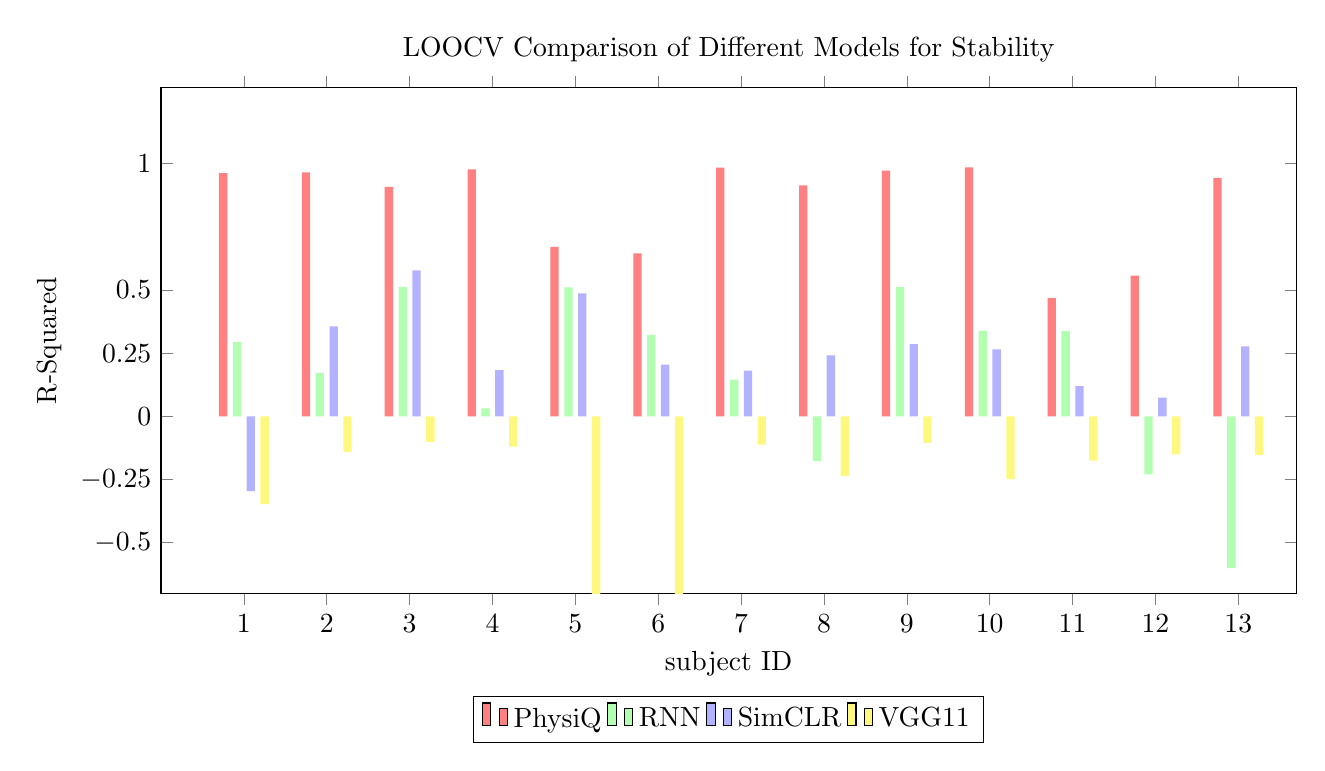
\begin{tikzpicture}
\begin{axis}[
    ybar,
    title=LOOCV Comparison of Different Models for Stability,
% 	x tick label style={
% 		/pgf/number format/1000 sep=},
	xlabel=subject ID,
	ylabel=R-Squared,
xtick={1,2,3,4,5,6,7,8,9,10,11,12,13},
ytick={-.5,-.25, 0, 0.25,  .5, 1.0},
% axis equal,
bar width=3pt,
height=8cm,width=16cm,
% 	enlargelimits=.1,
xmin=0, xmax=13.7, ymin=-.7, ymax=1.3,
	legend style={at={(0.5,-.25
	)},
	anchor=center,legend columns=-2},
% 	nodes near coords,  
%     nodes near coords align={vertical},  
% 	ybar interval=.4,
]
\addplot[draw=none, fill=red!50]  
%PhysiQ with attention
	coordinates {
	(1, 0.962759)
(2, 0.965883)
(3, 0.908476)
(4, 0.977755)
(5, 0.670809)
(6, 0.645153)
(7, 0.984199)
(8, 0.913709)
(9, 0.972433)
(10, 0.985297)
(11, 0.46807)
(12, 0.557421)
(13, 0.943878)
% python .\siamese_cross_validation.py --exercise sa --metrics stability  --lr .001 --hidden_size 256 --epochs 25 --dropout .2
% \begin{comment}
% average 0.8427571601500191
% (3, 0.962759, 0.00230378)
% (8, 0.965883, 0.0021105)
% (9, 0.908476, 0.00566173)
% (10, 0.977755, 0.00137607)
% (11, 0.670809, 0.020364)
% (12, 0.645153, 0.0219511)
% (13, 0.984199, 0.000977434)
% (14, 0.913709, 0.00533803)
% (15, 0.972433, 0.00170533)
% (16, 0.985297, 0.000909541)
% (17, 0.46807, 0.0329056)
% (18, 0.557421, 0.0273783)
% (19, 0.943878, 0.00347175)
% \end{comment}

};
\addplot[draw=none, fill=green!30]
	coordinates {
(1, 0.294923) 
(2, 0.17256) 
(3, 0.512831) 
(4, 0.0316302) 
(5, 0.510665) 
(6, 0.322193) 
(7, 0.145134) 
(8, -0.177127) 
(9, 0.511648) 
(10, 0.337905) 
(11, 0.337649) 
(12, -0.22917) 
(13, -0.600711) 
};

% average 0.16693313646634234
% (3, 0.294923, 0.0105827) 
% (8, 0.17256, 0.0124193) 
% (9, 0.512831, 0.00731207) 
% (10, 0.0316302, 0.0145346) 
% (11, 0.510665, 0.00734459) 
% (12, 0.322193, 0.0101734) 
% (13, 0.145134, 0.012831) 
% (14, -0.177127, 0.0176679) 
% (15, 0.511648, 0.00732984) 
% (16, 0.337905, 0.0099376) 
% (17, 0.337649, 0.00994145) 
% (18, -0.22917, 0.018449) 
% (19, -0.600711, 0.0240256) 
\addplot[draw=none, fill=blue!30]
	coordinates {
(1, -0.295405) 
(2, 0.356205) 
(3, 0.577606) 
(4, 0.183517) 
(5, 0.486332) 
(6, 0.204654) 
(7, 0.180871) 
(8, 0.241452) 
(9, 0.286067) 
(10, 0.265597) 
(11, 0.119688) 
(12, 0.0739067) 
(13, 0.276641) 
 };
\addplot[draw=none, fill=yellow!50] 
	coordinates {
(1, -0.347592) 
(2, -0.140759) 
(3, -0.101083) 
(4, -0.119998) 
(5, -0.735928) 
(6, -0.872492) 
(7, -0.111727) 
(8, -0.236336) 
(9, -0.104602) 
(10, -0.248734) 
(11, -0.174895) 
(12, -0.150518) 
(13, -0.152214) 
 };
	
\legend{PhysiQ, RNN, SimCLR, VGG11}

\end{axis}
\end{tikzpicture}
\caption{We also show the performance of shoulder abduction with the metrics of \textit{stability}. PhysiQ, shown in red, has perform significantly better than other models.}
\label{fig:stability}
\end{figure}


\subsubsection{Classification}
Next, we evaluate the PhysiQ's classification component on the quality of activity, i.e., how accurate can our model predict on \textit{ROMs}. Thus, our baselines for the models are some of the best classification models that modern machine learning and deep learning can achieve: CNN with Multi-Layer Perceptrons (MLP), LSTM with MLP, and Logistic Regression (Linear). Because classification and similarity comparison are two different problems, we target our problem using a different baseline but similar structure overall. CNN with MLP utilizes the 1-D Convolutional Neural Network to capture spatial knowledge and use the hidden representation to go through an MLP network to classify \textit{ROMs} and \textit{stability}. Similarly, LSTM with MLP has a similar approach, except a sliding windows segmentation is used to create a temporal representation, which feeds into the fully connected layer as MLP. Lastly, Logistic Regression is simply a fully connected model that considers all the points (dimensional flattening) in the signal and predicts the labels.

% \pgfplotsset{width=7cm,compat=1.8}
\begin{figure}
    \centering
    \includegraphics[width=\textwidth]{Data_figures/Figure2.png}
% \begin{tikzpicture}
% \begin{axis}[
%     ybar,
%     title= \change{LOOCV Accuracy  Among Different Models for Classifying Range of Motions Labels},
% % 	x tick label style={
% % 		/pgf/number format/1000 sep=},
% 	xlabel=subject ID,
% 	ylabel=Accuracy Percentage,
% xtick={1,2,3,4,5,6,7,8,9,10,11,12,13,14,15,16,17,18,19,20,21,22,23,24,25,26,27,28,29,30,31},
% ytick={ 0, .25,  .5, 1.0},
% % axis equal,
% bar width=1.5pt,
% height=6cm,width=16cm,
% % 	enlargelimits=.1,
% xmin=0,xmax=31.8, ymin=0, ymax=1,
% 	legend style={at={(0.5,-.35
% 	)},
% 	anchor=center,legend columns=-2},
% % 	nodes near coords,  
% %     nodes near coords align={vertical},  
% % 	ybar interval=.4,
% ]
% \addplot[draw=none, fill=red!55]  
% % python .\classification.py --exercise e1 --metrics rom  --lr .001 --hidden_size 256 --epochs 50 --dropout .2 --filename PHYSIQ_E1
% 	coordinates {
% (1, 0.9)
% (2, 0.98)
% (3, 0.98)
% (4, 0.92)
% (5, 0.92)
% (6, 0.82)
% (7, 0.96)
% (8, 0.94)
% (9, 0.96)
% (10, 0.88)
% (11, 0.9)
% (12, 0.76)
% (13, 0.94)
% (14, 0.98)
% (15, 0.9)
% (16, 0.96)
% (17, 0.88)
% (18, 0.64)
% (19, 0.9)
% (20, 1.0)
% (21, 0.96)
% (22, 0.86)
% (23, 1.0)
% (24, 0.86)
% (25, 0.84)
% (26, 1.0)
% (27, 0.88)
% (28, 0.78)
% (29, 1.0)
% (30, 0.94)
% (31, 0.98)


% };
% % python .\classification.py --exercise e1 --metrics rom  --lr .001 --hidden_size 256 --epochs 50 --dropout .2 --filename BASELINE_LOG_E1 --baseline log

% \addplot[draw=none, fill=green!30]
% 	coordinates {
% (1, 0.22)
% (2, 0.58)
% (3, 0.82)
% (4, 0.96)
% (5, 0.84)
% (6, 0.88)
% (7, 0.56)
% (8, 0.9)
% (9, 0.9)
% (10, 0.7)
% (11, 0.92)
% (12, 0.68)
% (13, 0.68)
% (14, 0.94)
% (15, 0.98)
% (16, 0.7)
% (17, 0.48)
% (18, 0.32)
% (19, 0.82)
% (20, 0.76)
% (21, 0.92)
% (22, 0.6)
% (23, 0.62)
% (24, 0.78)
% (25, 0.64)
% (26, 0.88)
% (27, 1.0)
% (28, 0.58)
% (29, 0.94)
% (30, 0.82)
% (31, 0.8)
% };
% \addplot[draw=none, fill=blue!30]
% coordinates {%python .\classification.py --exercise e1 --metrics rom  --lr .001 --hidden_size 256 --epochs 50 --dropout .2 --filename BASELINE_CNN_E1 --baseline cnn
% (1, 0.34)
% (2, 0.6)
% (3, 0.78)
% (4, 0.84)
% (5, 0.64)
% (6, 0.82)
% (7, 0.48)
% (8, 0.82)
% (9, 0.9)
% (10, 0.66)
% (11, 0.9)
% (12, 0.7)
% (13, 0.62)
% (14, 0.84)
% (15, 0.92)
% (16, 0.62)
% (17, 0.7)
% (18, 0.38)
% (19, 0.8)
% (20, 0.72)
% (21, 0.88)
% (22, 0.5)
% (23, 0.64)
% (24, 0.76)
% (25, 0.6)
% (26, 0.76)
% (27, 0.92)
% (28, 0.54)
% (29, 0.88)
% (30, 0.54)
% (31, 0.68)

%  };
% \addplot[draw=none, fill=yellow!50] 
% 	coordinates {%python .\classification.py --exercise e1 --metrics rom  --lr .001 --hidden_size 256 --epochs 50 --dropout .2 --filename BASELINE_RNN_E1 --baseline rnn
% (1, 0.48)
% (2, 0.58)
% (3, 0.72)
% (4, 0.66)
% (5, 0.62)
% (6, 0.52)
% (7, 0.76)
% (8, 0.36)
% (9, 0.74)
% (10, 0.44)
% (11, 0.56)
% (12, 0.6)
% (13, 0.62)
% (14, 0.8)
% (15, 0.6)
% (16, 0.64)
% (17, 0.52)
% (18, 0.24)
% (19, 0.4)
% (20, 0.8)
% (21, 0.52)
% (22, 0.38)
% (23, 0.56)
% (24, 0.42)
% (25, 0.32)
% (26, 0.68)
% (27, 0.48)
% (28, 0.32)
% (29, 0.32)
% (30, 0.56)
% (31, 0.56)

%  };
	
% \legend{PhysiQ, Logistic Regression, CNN,LSTM}

% \end{axis}
% \end{tikzpicture}
\caption{This figure shows the accuracy of our model with output of classification of \textit{range of motion}. As showed in this figure, our PhysiQ (shown in red) performs mostly better than the other models in this diagrams with a percentage accuracy on y-axis.}
\label{figure:loocv_class}
\end{figure}


As a result, we provide confusion matrices for all baselines and our model for classification of \textit{range of motion}. As shown in Figure   \ref{fig:sa_rom_classification:a}, \ref{fig:er_rom_classification:a}, and \ref{fig:ff_rom_classification:a}, compared against the other 3 baselines, our model demonstrates the best performance overall with a minimal inaccuracy on higher degree \textit{range of motion} exercises. The difficulties in differentiating between 30 and 60 degrees happen because of limited supervision and little self-reflection (such as a mirror), and all subjects might not perform homogeneously in the exercises. As a result, this might leads to inconsistency in the model to understand the difference between 30 degrees and 60 degrees ROM.

% \begin{table}[h!]
% \centering
% \begin{tabular}{||c | c | c | c | c||} 
%  \hline
%  Subject & PhysiQ  & Logistic Reg. & CNN & RNN \\ [0.5ex] 
%  \hline\hline
% 1   & 0.9333     & 0.7333    & 0.8   & 0.6333  \\ 
% 2   & 0.5       & 0.3667    & 0.6   & 0.4667  \\
% 3   & 0.7       & 0.7       & 0.6   & 0.4333  \\
% 4   & 0.6333    & 0.4667    & 0.5667& 0.5333  \\
% 5   & 0.9667    & 0.5667    & 0.7333& 0.6  \\
% 6   & 1.0       & 0.5667    & 0.5333& 0.4333  \\
% 7   & 0.7667    & 0.3333    & 0.7333& 0.4333  \\
% 8   & 0.5       & 0.5       & 0.4   & 0.3333  \\ 
% \hline
% avg & 0.7458    & 0.5292    & 0.6203& 0.4833  \\
%  \hline
% \end{tabular}
% \caption{LOOCV on Exercise External Rotation classification of \textit{range of motion}, with an average of 75\% accuracy on our models \meiyi{baseline?}}
% \label{table:er_class_rom}
% \end{table}
% python .\classification.py --exercise er  --lr .001 --batch_size 64
% percentage: 0.8
% (6, 1.0)
% (7, 0.7)
% (8, 0.733333)
% (9, 0.633333)
% (10, 0.966667)
% (11, 0.966667)
% (12, 0.966667)
% (13, 0.433333)\





% [todo: repetition classification]
% 
\begin{figure}
 \begin{subfigure}{0.24\textwidth}
     \includegraphics[width=\textwidth]{Figures/e1_physiq.png}
     \caption{PhysiQ}
     \label{fig:sa_rom_classification:a}
 \end{subfigure}
 \hfill
 \begin{subfigure}{0.24\textwidth}
     \includegraphics[width=\textwidth]{Figures/e1_baseline_logistic_regression.png}
     \caption{Logistic regression}
     \label{fig:sa_rom_classification:b}
 \end{subfigure}
 \hfill
%  \medskip
 \begin{subfigure}{0.24\textwidth}
     \includegraphics[width=\textwidth]{Figures/e1_baseline_cnn.png}
     \caption{CNN}
     \label{fig:sa_rom_classification:c}
 \end{subfigure}
 \hfill
 \begin{subfigure}{0.24\textwidth}
     \includegraphics[width=\textwidth]{Figures/e1_baseline_lstm.png}
     \caption{RNN}
     \label{fig:sa_rom_classification:d}
 \end{subfigure}

 \caption{This is the confusion matrices for classification of \textit{range of motion} in \textbf{shoulder abduction} with PhysiQ and baselines. Shoulder abduction has class of 5 from 30, 60, 90, 120, and 150, which is labeled from 0 to 4}
 \label{fig:sa_rom_classification}

\end{figure}


\begin{figure}
 \begin{subfigure}{0.24\textwidth}
     \includegraphics[width=\textwidth]{Figures/e2_physiq.png}
     \caption{PhysiQ}
     \label{fig:er_rom_classification:a}
 \end{subfigure}
 \hfill
 \begin{subfigure}{0.24\textwidth}
     \includegraphics[width=\textwidth]{Figures/e2_baseline_logistic_regression.png}
     \caption{Logistic regression}
     \label{fig:er_rom_classification:b}
 \end{subfigure}
 \hfill
%  \medskip
 \begin{subfigure}{0.24\textwidth}
     \includegraphics[width=\textwidth]{Figures/e2_baseline_cnn.png}
     \caption{CNN}
     \label{fig:er_rom_classification:c}
 \end{subfigure}
 \hfill
 \begin{subfigure}{0.24\textwidth}
     \includegraphics[width=\textwidth]{Figures/e2_baseline_rnn.png}
     \caption{RNN}
     \label{fig:er_rom_classification:d}
 \end{subfigure}

 \caption{This is the confusion matrices for classification of \textit{range of motion} in \textbf{external rotation} with PhysiQ and baselines. The external rotation has a class of 3 from 45, 90, and 150, which is labeled from 0 to 2}
 \label{fig:er_rom_classification}

\end{figure}

\begin{figure}
 \begin{subfigure}{0.24\textwidth}
     \includegraphics[width=\textwidth]{Figures/e3_physiq.png}
     \caption{PhysiQ}
     \label{fig:ff_rom_classification:a}
 \end{subfigure}
 \hfill
 \begin{subfigure}{0.24\textwidth}
     \includegraphics[width=\textwidth]{Figures/e3_baseline_logistic_regression.png}
     \caption{Logistic regression}
     \label{fig:ff_rom_classification:b}
 \end{subfigure}
 \hfill
%  \medskip
 \begin{subfigure}{0.24\textwidth}
     \includegraphics[width=\textwidth]{Figures/e3_baseline_cnn.png}
     \caption{CNN}
     \label{fig:ff_rom_classification:c}
 \end{subfigure}
 \hfill
 \begin{subfigure}{0.24\textwidth}
     \includegraphics[width=\textwidth]{Figures/e3_baseline_rnn.png}
     \caption{RNN}
     \label{fig:ff_rom_classification:d}
 \end{subfigure}

 \caption{This is the confusion matrices for classification of \textit{range of motion} in \textbf{forward flexion} with PhysiQ and baselines. Forward flexion has a class of 5 from 30, 60, 90, 120, and 150, which is labeled from 0 to 4}
 \label{fig:ff_rom_classification}

\end{figure}


\subsection{Parameters Evaluation}\label{evaluation:subsec:parameters}
\subsubsection{Sliding Windows}
To evaluate the accuracy of our proper performance, we use different sliding window segmentation of samples to test our model results. We test the performance on leave-one-subject-out cross-validation (LOOCV). By having sliding windows that are 50, 100, and 150. The model decreased its performance when the sliding windows increased while keeping the same step size. Increasing the sliding window size decrease the number of time, or redundancy, for the model to see. Having smaller sliding windows helps the model to understand the quality of exercises. At the same time, as we increase the step size (the size of overlapping), the model also performs better but sees a drop in the testing dataset. An extensive redundancy overfits the training distribution and does not generalize it well. As a result, we choose a sliding window of 50 with a step size of 15 for training, validating, and testing, which alike to our data collection rate of 50 Hz. Having some redundancy helps the model to generalize the relationship between sliding windows.

\subsubsection{Repetition Size}
In repetition size, we have a different size in similarity comparison. We have each ID number of segmented exercises for each subject. Adjacent ID number represents that they can be concatenated together to output different. We use the same number of repetition sizes in training and testing. The model has a slight difference in accuracy (3 - 5 percent) in bigger repetitions as length increases. However, this is also affected by the hyperparameters that we choose. Without changing the step size and window size, the model can still perform well because our model generalizes very well. Moreover, we also see a performance increase when adding dropout regularization deep LSTM network. As a result, the performance of four repetitions becomes 0.921 in the R-Squared correlation.


\subsubsection{Padding}
We also evaluate the effect of front padding and back padding. We hypothesize that there should be no difference between front and back padding. However, when the padding is at the end of the temporal sequence, the model does not learn, resulting in an average R-Squared score of 0. Moreover, the results remain unchanged throughout the epochs. This non-learning behavior happens possibly due to the fact that many of the segments are varied significantly. In that cases, many of the windows remain zero and do not help the model to learn. At the same time, as we attempt the model without padding or minimize the amount of padding, we are facing the issue that the temporal model could cheat the result because there is a correlation between higher \textit{range of motion} exercises and the length of the data. In contrast, lower ROM exercises can have a shorter overall length. This relation could result in an accumulating effect of shortcuts for the deep learning model to learn and cheat. So using constant front padding for all one repetition exercises is consistent and performs similarly in a different number of repetitions.  
% [TODO: Would it be more convincing to have random noises]
% [TODO: Cross Validation on Padding]
\subsection{Ablation Study}\label{evaluation:subsec:ablation}
\subsubsection{Removal of Hidden Representations} 
After removing the \textbf{temporal representation}, LSTM encoder, part of PhysiQ, the model still performs relatively well with an MSE 0.007168, MAE 0.0665, and R-Squared 0.8346 with 256 hidden features. At the same time, we did the same procedure for \textbf{spatial representation}. After removing the CNN encoder from PhysiQ, the model performs relatively well with an MSE 0.00873, MAE 0.063, and 0.8208 in R-Squared with one hidden temporal layer and no dropout regularization. Interestingly, in the usages of both spatial and temporal models, our model can achieve 0.92 R-Squared while removing either of them drops significantly by around 10 percent. The decrease happened due to the reasoning that the signal data contain both spatial and temporal information, and a single model can only capture part of the information with the help of an attention mechanism. 
\subsubsection{Dropout}
% python .\siamese_cross_validation.py --exercise sa --metrics rom --hidden_size 256 --batch_size 1024 --num_layers 1 --dropout 0 --epochs 50 --filename dropout_0_evaluation
Testing the dropout is also essential to see how the model is generalized. This dropout is applied in every layer, including the spatial encoder (CNN) and temporal encoder (LSTM). We used LOOCV to compare our results with 0\%, 20\%, and 50\% dropout rates to see if the difference is significant. We test our model with hidden features of 256 for temporal and spatial encoding, two LSTM layers, 16 heads of attention, and a batch size of 1024. The model should not have a significant difference between 20\% and 50\% but possibly a slight performance boost in 20\% or 50\% compared to 0\%. Our model is meant to generalize well across participants and should not overfit the training distribution; the average result of 0 percent dropout across the participants is 89.66\%. The average result with 20 percent dropout is 89.73\%. The average result with 50 percent dropout is 87.87\%. Interestingly, the 20\% dropout rate generates a slightly better results than 50\%.  This is because 20\% has already created its maximal regularization for the model, and increasing the dropout rate does not benefit from regularization. On the other hand, a much higher dropout rate could result in a higher variance in the model, resulted degradation in performance. Having only a 20\% dropout rate creating the maximum of regularization makes our model more convincing in terms of generalizability. 

\subsubsection{Attention}
We test the importance of attention in our model. Attention is applied to selectively focus on more critical aspects of the input sequence. In our model, attention is a final layer to measure the relationship between each hidden state. With that in mind, we remove the attention layer to compare results in the metrics of the \textit{range of motion} in shoulder abduction, external rotation, and forward flexion. Without the attention layer, the performance of LOOCV in shoulder abduction drops to a 0.892 R-squared correlation from 0.908. On exercise external rotation, the performance of LOOCV drops to a 0.560 R-squared correlation from 0.675. Meanwhile, the performance of LOOCV on forward flexion has an insignificant increase from 0.815 to 0.830. In summary, if the motion data is distinguishable and representative, the attention layer does not have a huge impact. However, when exercise has a limited motion, such as half-half arm span exercise external rotation, the attention layer is more impactful.

% [todo: LSTM with one layer does not apply dropout, change it to two if it is possible?] Yes and better!
% (1, 0.0791741)
% (2, 0.672945)
% (3, 0.647328)
% (4, 0.198096)
% (5, 0.721232)
% (6, 0.707202)
% (7, 0.879687)
% (8, 0.935965)
% (9, 0.740117)
% (10, 0.657246)
% (11, 0.753034)
% (12, 0.852191)
% (13, 0.8029)
% (14, 0.952477)
% (15, 0.765612)
% (16, 0.73964)
% (17, 0.887934)
% (18, 0.923182)
% (19, 0.567274)


% \subsection{A Second Exercise: External Rotation}
% We test the \textit{range of motion} metrics of external rotation exercises to support our model's performance. However, segmenting the exercise repetitions is more difficult because the energy of external rotation is significantly lower than shoulder abduction due to its travel distance. Therefore, we have segmented using different parameters for our energy method; we use [1, 0.2, 1] on the weights, dropping the y-axis' importance in producing the energy and changing $\lambda$ to be 0.7, which means the neighbor energy are weighted less. Unfortunately, due to limited time, we have \change{20} participants for three different sets of exercises (45, 90, and 150 in range of motion) to validate our model's generalizability. Interestingly, adding 20\% percent of dropouts can help generalize the model better in testing. It is because due to the different data distribution, dropout acts as a regularization to help better alleviate covariate shift from the testing data. In addition, we discover that subject 8 has the slowest movement speed compared to all other subjects, which explains why the model does not learn in LOOCV when testing subject 8 because the model has never seen this subject's exercise. For example, subject 8 has around 150 data points (3 seconds) compared to other subjects with only 100 data points (2 seconds) with the same ROM. Therefore, it is likely to become a covariate shift when the model is trained based on the first seven subjects and has not seemed to the distribution of subject 8.

% Moreover, we also test using 70-10-20 normal evaluation to test the overall performance. Overall, in 10 test runs, our result of similarity comparison is \change{0.0117 for MSE, 0.0882 for MAE, and 0.757} for R-Squared. Additionally, we test our model with LOOCV on the classification output of ROM, which resulted in an average of \change{83.860}\% accuracy over all subjects. Interestingly, the classification accuracy generates a similar output compared with the R-Squared similarity comparison, that subject 8 has the lowest prediction accuracy.
% \change{
% \subsection{A Third Exercise: Forward Flexion}
% We test the \textit{range of motion}, \textit{stability}, and \textit{repetitions} metrics of forward flexion exercises to further evaluate our model's performance. In order to segment this exercise, we use slightly different parameters compared to shoulder abduction while they are similar in actions. We segment the data using [1, 0.01, 0.8] on the weights, dropping the y-axis' importance and narrowly alleviating the z-axis, and we change $\lambda$ to be 1, making the neighbor energy to be more vital. 
% We have 12 participants in  forward flexion for five sets  (30, 60, 90, 120, and 150 in the range of motion). IN 70-10-20 for \textit{range of motions}, we have a performance of MSE of 0.00215, MAE of 0.0366, and R2 of 0.950. Similarly, in \textit{stability} we have a performance of MSE of 0.00602307, MAE of 0.0594639, and R2 of 0.883. Additionally, in LOOCV, for \textit{repetitions} of \textit{range of motion}, we have 0.8137, 0.8363, and 0.9018 in repetitions 1, 2, and 3 respectively. Interestingly, forward flexion's performance is slightly better than external rotation. Forward flexion and shoulder abduction are part of half arm span exercises with a greater traveling distance of motion in the arm. However, the external rotation has a smaller distance of motion that might make the model harder to understand the underlying structure through supervised learning.}
% classifcation accuracy:
% percentage: 0.6625
% (6, 0.9)
% (7, 0.4)
% (8, 0.633333)
% (9, 0.633333)
% (10, 0.933333)
% (11, 0.966667)
% (12, 0.6)
% (13, 0.233333)

% \begin{table}[h!]
% \centering
% \begin{tabular}{||c c c||} 
%  \hline
%     Subject & R-Squared & MSE \\  [0.5ex] 
%  \hline\hline
%     1 &     0.68336    & 0.0187787    \\ 
%     2 &     0.226178   & 0.0458925  \\
%     3 &     0.300519   & 0.0414836  \\
%     4 &     0.427823   & 0.0339337  \\
%     5 &     0.792675      & 0.0122956 \\
%     6 &     0.792591     & 0.0123007  \\
%     7 &     0.76821   & 0.0137466  \\
%     8 &     0.192196   & 0.0479078   \\
%  \hline
% \end{tabular}
% \caption{Similarity Comparison Results with External Rotation Data}
% \label{table:ER_crossvalidation_Result}
% \end{table}
% Adam optimizer
% python .\siamese_cross_validation.py --exercise er --lr .001 --dropout .2 -- num_layer 2
% average 0.5229439409029432
% (6, 0.68336, 0.0187787)
% (7, 0.226178, 0.0458925)
% (8, 0.300519, 0.0414836)
% (9, 0.427823, 0.0339337)
% (10, 0.792675, 0.0122956)
% (11, 0.792591, 0.0123007)
% (12, 0.76821, 0.0137466)
% (13, 0.192196, 0.0479078)




% train on one exercise and test on other exercise
% train on 1 repetition and test on more than 1 repetition
% varied length comparison? do we need padding?


%\subsection{Principle Component Analysis (PCA) Visualization of Model Representation}

% PhysiQ 0.00619457 mae 0.0627772 r2 0.85198
% SimQLR mse 0.0104795 mae 0.0785231 r2 0.757808
% VGG contrastive mse 0.0469153 mae 0.179209 r2 -0.0817496

%
% input_size=6, hidden_size=256, num_layers=1, batch_size=256, batch_first=True, attention_flag=True, width=50, step=15, bidirectional=False, num_heads=16, total_length=1550, cnn_kernel_size=3, output_size=5, dropout=0.0, lr=0.0001, epochs=50, decoder_mode='siamese', sub_info=False, test=False, num_reps=5)


% Shoulder abd stability:
% 	- Cross validation table
% 	- 70-10-20 table
	
% External rotation rom:
% 	- Cross validation table
% 	- 70-10-20 table

% MLP:
% Baseline:
% 	- Random Forest
% Different variation:
% 	- CRNN
% 	- CRNN + CNN
% 	- CRNN + CNN + Attention
% Shoulder abd rom:
% 	- Classification confusion matrix
	
	
% Shoulder abd stability: 
% 	- Binary or classification (ROC or confusion matrix)

% External rotation rom:
% 	- Classification confusion matrix



\section{A Survey on User Experience}
\label{sec:survey}

To investigate PhysiQ's application in practice, we surveyed the participants who used our system for data collection. Users wear an Apple Watch with a connected iPhone with our PhysiQ apps installed during data collection. In the beginning, users have the exercise instruction on the phone to start. 
% Next, users tap the start button on the smartwatch, and the smartwatch counts 3 seconds down and gives a vibration as a signal to the users to start exercising. Afterward, they press the stop button to transfer the session data to the iPhone. 
PhysiQ on the phone visualizes the signal to see the repetition quality and feedback to the users (as shown in Fig. \ref{fig:PhysiQ_GUI}). 

After collecting the data, we distribute a questionnaire to all users. The questionnaire asks six questions on different scales. 
We designed the survey questions for three purposes. First, we get users' feedback on our current design (Q1). Secondly, we explore users' preferences in alternative platforms and recommendations to improve our current design (Q2 and Q3). Last, we gather users' demographic information (presented in Section \ref{sec:data collection}) and ask behavioral questions (Q4-Q6). We study the correlation between users' behaviors and the performance of our algorithms in measuring their activities. 
We attach the questions and summary of results below because we believe our findings are valuable for our future work and the research community. 

\begin{itemize}
    \item \textbf{Q1: How do you like the current feedback and recommendation system?} 
        \begin{itemize}
        \item scale of 1 to 5, with 1 being the lowest, and 5 being the highest
        \end{itemize}
    \item \textbf{Q2: If we have a different platform, what platform will you like to have recommendation system of the exercises on?}
        \begin{itemize}
        \item Smartwatch
        \item Smartphone
        \item Smartglasses such as VR, AR glass
        \end{itemize}
    \item \textbf{Q3: During what period of the exercise do you like such feedback? For example, for today's exercise session, you have 5 different exercises to perform and for each exercise, you have 10 repetitions of 5 sets? }
        \begin{itemize}
        \item After a set of exercises  (during this particular exercise, after 10 repetitions)
        \item After the particular exercise of 5 sets
        \item After the entire exercise session (after 5 exercises)
        \end{itemize}
    
     \item \textbf{Q4: During the time of collecting your exercise data, do you drink coffee or any caffeinated drinks regularly? If so, how often? }
        \begin{itemize}
        \item Every day
        \item A few times a week
        \item About once a week
        \item A few times a month
        \item Once a month
        \item Less than once a month
        \end{itemize}
    
    \item \textbf{Q5: During the time of collecting your exercise data, how many hours do you sleep? } 
        \begin{itemize}
        \item Time in hour
        \end{itemize}
        
    \item \textbf{Q6: This question is regarding your medical history and you do not need to specify the medication. At the time of collecting your exercise data, do you know and take any medication at the time that would affect your ability to perform exercise or activity? }
        \begin{itemize}
        \item Yes or no
        \end{itemize}
    \end{itemize}
    
Out of 31 participants, we have 27 participants who complete the follow-up survey. Overall, we have an average of 4.26 rating on how much the users like our system. Interestingly, we have 48.1\% of the users who want to have a recommendation on a smartwatch, 51.9\% of the users on a smartphone, and no one wants to use smart glass to get recommendation feedback. Additionally, 59.3\% of our users want to have their feedback after a set of exercises, 22.2\% after the particular exercises, and 14.8\% after an entire session. Lastly, one participant suggests they should be able to see the feedback anytime they want.

Moreover, we have 18.5\%, 33.3\%, 14.8\%, 18.5\%, 3.7\%, and 11.1\%, respectively, on the frequency of coffee consumption based on the answer order above. At the same time, on average, our participants sleep 7.63 hours with a minimum of 6 and a maximum of 9. Lastly, we only have 1 participant possibly on medication that affected their performance overall, but we do not find that medication was affecting the performance of our model testing on this participants' exercises.



    




\section{Discussion}
\label{sec:discussion}

\subsection{Applications}
\emph{Physical Therapy Home Assessment}. This application is intended to work for patients and people injured, postoperative, or mentally traumatized. While performing at-home exercises, our application can provide real-time feedback and assess the quality of the exercises to provide better interaction and supervision while clinics are not accessible. At the same time, we believe our model is capable of analyzing and predicting people who might suffer from a different illness or potential injuries. One example is that people with heavy usage of handcrafting might suffer from carpal tunnel syndrome, which is caused by pressure on the median nerve. 

\emph{Daily Exercises Assessment}. This application can also support working with people who enjoy exercise. People can benefit from it by closely assessing how they perform specific repetitions of exercises. Moreover, this application could also apply to people who are playing sports. We envision that our model can eventually support people who play sports like tennis to predict a player's direction, speed, or posture.


\subsection{Assumption and Limitation}
This paper discusses the potential of using a smartwatch to support users assess their exercises with a quantitative measure of the quality. However, there are a few assumptions made to support this application. First of all, we assume that the users' posture should have some level of decency. For example, suppose users perform the exercise of shoulder abduction while bending their neck or wiggling around as not in a straight form. In that case, the application likely can still give a good score on the exercises simply because the users might still perform the exercise correctly. Because the smartwatch cannot capture all the movement within the body, we do not have the luxury of analyzing all the posture. Secondly, 
we assume that the primary segmentation is performed upon accelerometer data, and its energy is only extracted from the accelerometer. Thirdly, 
we assume there is 5 level of quality of exercises in \textit{range of motion} in shoulder abduction. These are our metrics to digitalize from body movement to computational numbers. The five levels can vary based on different professionals' metrics, and our goal is to standardize a metric in our model that can measure and understand.


% \subsection{Limitation}
% PhysiQ is a new framework that has the potential to generalize to different tasks in various exercises. However, there are some limitations to our project. 
We notice that the energy plot does not have a clear pattern in some exercises for some subjects. Such limitation is due to our little knowledge regarding the data collection. Applying our energy plot when collecting data from the users could be more rigorous and use it as a checkpoint to verify if the subjects have correctly performed the exercises.
% Moreover, there is a problem of imbalanced data among the actual patients and healthy participants due to the limited resource and time. We do not have the luxury of collecting data from actual patients. Thus, our model is limited to testing only on the people who did not have injuries at the time. 
% We also observe that the participants' speed in performing the exercise can affect the performance of the models. One potential solution is to augment the dataset to expand or shorten the length of segments. Additionally, we define a metrics of \textit{range of motion} in scale of 30, 60, 90, 120, 150. Discrete classification can be a limitation due to the inconsistency of participants' movements. We observe and judge the participants' range of motion visually. However, we could standardize the method by using a regression method from a 3-D motion projectile. 
In the future work, we will improve our framework to better handle above assumptions and limitations.  

\section{Summary}
\label{sec:summary}

% \meiyi{replace this para with a 'summary':}
% This paper focuses on exploring and analyzing the performance of our model and exploiting current technologies. Furthermore, we believe this area has many potentials, including 1. using the self-supervised method because of the limited data collection, 2. unsupervised learning to generate features that professionals could use, 3. reinforcement learning method to recommend different sets of exercises to perform depends on the users' short-term and long-term goals, and 4. creating an innovative method to segment exercises of different kinds through deep learning methods dynamically. 

% \meiyi{below is fine}
We develop an innovative system, PhysiQ, to quantitatively digitalize the quality of exercises through new metrics on a commodity smartwatch. We scrutinize and verify that different metrics and exercises have unique characteristics that can be recognized and understood by our deep learning model. By developing such a model based on Siamese Neural Network with additional spatiotemporal representation encoding, our model can achieve 95 percent R-square correlation and 90 percent accuracy in classification. Moreover, a comprehensive evaluation and user studies are performed to show the effects on our metrics in range of motion, stability, and repetition. 
The end goal is to improve the prediction and assessment of people who needs therapy to improve their quality of life. In addition, we envision that current technologies and relevant professions can be benefited from it by expanding usability, generalizability, and model learnability. By combining deep learning and the physical therapy method, we believe that our framework is the tool to lead people to improve their quality of life.

\section{Acknowledge}
This work was supported in part by National Science Foundation 2220401. We would also like to thank Zirong Chen, Xing Yao, David Atwood, Melissa Wang, Anna Chen, and Yashvitha Thatigotla for their effort to help and discuss this project.
% We would like to thank Zirong Chen and Xing Yao for the intercommunication on design and technical support. We would also like to thank our undergraduate research assistants, David Atwood, Melissa Wang, Anna Chen, and Yashvitha Thatigotla, for their effort to help and discuss our project.

\bibliographystyle{ACM-Reference-Format}
\bibliography{sample-base}

% \newpage
% \Large
\noindent\textbf{Response Letter} \\
\label{rev:response}
We truly appreciate all the valuable comments from the reviewers. We have done a major revision on the paper to address all the comments. We highlighted the revised parts using blue text in the paper. 
To answer the reviewer’s questions, we write a response to each comment below. 

Additionally, we summarize the changes below:
\change{
\begin{itemize}
    \item We significantly increased our collected dataset. (1) We nearly doubled the participants in all exercises and added a third exercise, forward flexion. (2) The third exercise underwent the same procedure and evaluation as the first two, and significantly outperformed the baselines, which further confirmed the generalizability of our model, PhysiQ. (3) We provided figures and explanation on why we choose this exercise, forward flexion in Fig. \ref{fig:Exercises}, Page \pageref{fig:Exercises}. (4) With a total of three exercises and three metrics, we expanded the age range between 19 and 44 with more survey completion. 
    \item (1) Based on our in-depth analysis of muscular system and difference among arm-spans, we appended a new ground truth section to explain our labeling procedure for the range of motion and stability. We explained the reasoning for how we get stability and range of motion in Sec. \ref{subsec:solution:digitalizingExerMetrics}, Page \pageref{subsec:solution:digitalizingExerMetrics}. (2) With the modification of stability ground truth, we conducted our evaluation on all exercises. As a result, in all three exercises metrics, our model significantly outperformed all baselines and showed that with a sophisticated design of metrics, our model learns the underlying structure of the signals.
    \item We added a problem formulation section to define our problem of supervised learning. We explained the classification and similarity comparison problems separately in Sec. \ref{subsec:solutions:problem}, Page \pageref{subsec:solutions:problem}. 
    \item We improved our mobile application to demonstrate the structure of the PhysiQ framework with additional screenshots in Fig. \ref{fig:PhysiQ_GUI}, Page \pageref{fig:PhysiQ_GUI}. We also showed the potential of our framework in real-life scenarios between patients and doctors.
    \item We re-conducted the evaluation section with expanded datasets and re-evaluated the results with extensive tables and figures. Our model demonstrated the generalizability in different participants, metrics, and exercises. PhysiQ also outperformed the baselines as a backbone to classification problem of range of motion. 
    \item We carefully checked the manuscript and adjusted the description accordingly, as suggested by the reviewers.
\end{itemize}
}
\vspace{0.5cm}
\noindent\textbf{1AE's meta-review (Reviewer 2)}
\begin{itemize}
    \item Increasing the experimental data sample size 
    
    \change{We collected 11 more participants data, aged between 19 and 44. Additionally, we also added another exercise, forward flexion, to be part of this work.}
    \item Formal problem definition and important representation: we believe that using deep learning methods, it can helps patients and therapists to understand the quality of exercises through defined metrics and fathom the nuances of exercises they performed. 
    
    \change{We added a section of formal problem definition in Sec. \ref{subsec:solutions:problem}, Page \pageref{subsec:solutions:problem}}
    \item New results on "range of motion" and "stability" 
    
    \change{New results and evaluation has been updated in Sec. \ref{sec:evaluation}. We re-ran most of the evaluation because of the expansion of the dataset.}
    \item Clear description of the ground truth 
    
    \change{We added a ground truth section in Page \pageref{subsec:solution:digitalizingExerMetrics}, Sec. \ref{subsec:solution:digitalizingExerMetrics}.}
    \change{And we modified the metrics of \textit{stability} to make our model more accessible.}
    \item Improving the writing quality

    
    \change{We re-checked and re-read everything. Thank you for all the suggestions.}
\end{itemize}


\large
\noindent\textbf{2AE (Reviewer 1)}
\begin{itemize}
    \item The manuscript has some detailed description errors
    
    \change{We re-read and correct as many errors as we think we have made. Thank you for the suggestions!}
    \item Is the dataset too small? Since smartwatch is a convenient device to collect data, it should collect more datasets of participants who are injured or increase normal participants who are not injured and simulate the stability. 
    
    \change{We collected 12 more participants and re-defined the metrics for stability to be useful across all dataset.}
    \item There is a lack of description of shape of input data and problem definition in the methodology. Problem definition with data dimension transformation will make the process of spatio-temporal feature representation more specific.  
    
    \change{We clarified our dimensions, problem definitions, and methodology in Sec \ref{sec:data collection} and Sec \ref{sec:solutions}}
    
    \item Following the weak point 1, for instance, there is a grammar error in the
    caption of Fig. 3: “Exercises Metrics: we first identify the type of exercise to
    perform and that model measures the quality of.”. Additionally, The description of
    Table. 2 are mis-presented. More details need to be check in the manuscript.
    
    \change{We fixed it accordingly, and re-visited all the manuscripts. Thank you for your suggestion!}
    \item Following the weak point 2, considering that people in Previously Shoulder
    Injures are not easy to find, this can increase the dataset as much as possible.
    
    \change{We re-conducted and re-visited the data collection process, and collected 12 participants with 3 exercises. Based on that, we ran the evaluation with all three metrics of range of motion, stability, and repetition.}

\end{itemize}
\large

\large
\noindent\textbf{Reviewer 3}
\begin{itemize}
    \item How does the method distinguish "range of motion" and "stability"? Does it utilize the energy method? If yes, can you show the experiment result of it? If not, please clarify this. 
    
    \change{It does not utilize the energy method; we clarified it in the ground truth section in Page \pageref{subsec:solution:digitalizingExerMetrics}, Sec \ref{subsec:solution:digitalizingExerMetrics}. Energy method is used to segment repetitions in a session. Range of motion is labeled with physical movement, and stability is measured through coefficient of variation.}
    \item The description of the Spatio-temporal Feature Representation is not clear. What is signal exercise and anchor exercise? Are they two consecutive exercises?
    
    \change{The signal exercise is user's new exercise that is been done and used to compared the "perfect" anchor exercise. These two are not consecutive exercises.}
    \item How is the ground truth of similarity score defined? Please provide an example for clarification.
    
    \change{The ground truth of similarity score, stability and range of motion is defined in Page \pageref{eq:rom} and Page \pageref{eq:stb} in Equation \ref{eq:rom}, \ref{eq:stb}.}
    \item In the classification experiment (section 5.4.2), there is no figure for stability. Please provide the description and figure for it. 
    \change{We modified our ground truth and stability is now between 0 and 1. We have shown our result of three metrics in table \ref{table:sa_701020}. }
    \item The sample size is small and the range of age is also small. It will be more representative if the dataset is larger. 
    
    \change{We increased our dataset by adding 12 participants and add another exercise to evaluate our model.}
\end{itemize}

\large
\noindent\textbf{Reviewer 4}
\begin{itemize}
    \item Paragraph 1 of Introduction: it would be better to motivate this work and explain the impacts by citing some numbers, e.g., how many people could benefit from PT. 
    
    \change{We added such motivation in the introduction. Thank you for your suggestions!}
    \item line 38, this claim came out of nowhere, i.e., why do we start directly from deep learning? Why don't naive solutions work here? 
    
    \change{We re-structured and re-phrased the motivation section along with the second part of the introduction due to inconsistency of the context.}
    \item Section 1.1, it's unclear how this work differs from the existing works mentioned in previous paragraphs, e.g., no related work is cited in the section.  
    
    \change{We added the reference of works and added our work is focus on to let patients' see their quality of exercises through muscular metrics.}
    
    \item line 69-70, grammar mistake: "there do not have" 
    
    \change{We fixed it accordingly. Thank you for the correction.}
    \item line 79, similarly, there is no justification for starting with deep learning models. 
    
    \change{We re-structured and re-phrased the motivation section along with the second part of the introduction due to inconsistency of the context.}
    \item It would be good to mention how does this work address these mentioned challenges.
    
    \change{We re-stated how our work helps to target the aforementioned challenge in the introduction. The list of contributions corresponds to the challenges. }
    \item In introduction, there should be a lot of motion tracking papers at least, which may not be focusing on professional metrics but they should be mentioned.
    
    \change{We mentioned more papers of HAR in the introduction as suggested, including ones on how to improve the quality of life through smart HAR.}
    \item  Line 97, it's hard to justify this novelty since there are already mature products doing this such as Apple Watch or Switch. They may have not have paper published but there should be plenty of patents. 
    
    \change{We double checked that there is no product on recognizing the quality of exercises but number of steps, calories, and potentially arm position. But these results do not consider as quality of exercises through muscular metrics. First bulletin point in contribution in introduction updated to mention our work is not just about similarity, but also a comparison of quality of metrics.}
    \item The contribution list is not well organized, e.g., collecting data is trivial considering the size of the data. 
    
    \change{To address this comment, we added another 12 participants across the existing two types of exercises, and added one additional exercise, forward flexion. The challenge and novelty of our data collection is that we collect and annotate the data with different levels of quality per different metrics.}
    \item line 197, the muscular system is not even mentioned in the introduction? It should be since it seems to be a major novelty of this work.
    
    \change{Thank you very much for this detailed suggestion. We presented our idea of the muscular system in Sec. \ref{sec:solutions}, and we also added muscular system as a basis to our exercises metrics in the contribution list. }
    \item  line 310, "we use our intuition to decide on the cutting point for segmentation", this is so not convincing. 
    
    \change{We explained accordingly in the Sec. \ref{subsec:solution:digitalizingExerMetrics}, that we used the previous and next repetition as a neighbor energy to amplify the cutting point.}
    \item line 314, how are the labels collected? 
    \change{We clarified it in the ground truth section in Page \pageref{subsec:solution:digitalizingExerMetrics}, Sec \ref{subsec:solution:digitalizingExerMetrics}.  Range of motion is labeled with physical movement, and stability is measured through coefficient of variation.}
    
    \item line 317, is "shoulder abduction exercise" used as an example or is it the only exercise considered? 
    
    \change{We used shoulder abduction as the primary example to test our model but added two more exercises to assess more.}
    
    \item line 345, figure 6 is far away from this line.
    
    \change{We modified the location of figure 6 to be closer to the actual paragraph.}
    \item line 346, citation for the mentioned similar work. Also, it is worth explaining the difference. 
    
    \change{We added citations and explained the differences in the later section in SNN.}
    \item line 354, CNN is used without justification.
    
    \change{We justified CNN as our spatial compression model to represent information in each sliding windows.}
    \item line 399, reference missing.
    
    \change{We added the reference of LSTM as suggested.}
    \item line 549, the two exercises should be mentioned in the introduction.
    
    \change{We mentioned all three shoulder exercises in the introduction section.}
    \item Section 5.4.1, the choice of baselines should be better explained at the beginning of the paragraph. 
    
    \change{We added our reasoning for RNN, CNN and SimCLR with its reference. RNN and CNN because RNN is known for arbitrary input with time-varied data, and CNN learns well in spatial and temporal features. Additionally, we choose SimCLR as third baseline because its architecture enables useful representation learning in contrastive learning.}
    \item Section 5.6, why not show the ablation for the attention layer?
    
    \change{We added an attention ablation study for our model.}
    \item line 725, how will you deploy and update your model to the app? E.g., based on Figure 1.
    
    \change{We envision to deploy our deep learning model into cloud server to support API call directly from our mobile application. It is also easy for update and version control.}
\end{itemize}
\end{document}
\endinput

%%
%% End of file `sample-manuscript.tex'.
